\section{Signal Efficiency Systematic Uncertainties \label{sec:SystUnc}}

The signal efficiency for all the analyses is determined from MC simulation. To assess how well simulation matches data, numerous studies were performed using control samples.
The largest uncertainty for most of the signals is the trigger efficiency uncertainty. For low mass samples, the uncertainty on the selection variables becomes
dominant as the HSCPs become more relativistic. For multiply charged samples, the uncertainty on the amount of material in CMS, which affects the fraction of $Q>e$ particles
that stop before the muon system, is dominant.

\subsection{Trigger Efficiency Uncertainty}


The uncertainty on the muon trigger efficiency can come from numerous different effects. 
A 5\% difference in the muon trigger efficiency has been observed between data and MC simulation~\cite{2012JInst...7P0002T}.
An additional uncertainty important to slow moving particles is the timing synchronization in the muon system. As an HSCP arrives in the muon system
closer to the switching of the assigned bunch crossing window, a discrepancy in the modeling of the timing synchronization in the MC simulation
would have a larger effect than for SM particles.

As discussed in Section~\ref{sec:trigtime}, the trigger timing of the CSCs is determined at the chamber level. In a similar way,
the trigger timing for the DTs and RPCs are also determined at the chamber level.
The average and RMS of the synchronization of the chambers with respect to the LHC clock was measured for each subsystem.
For the CSCs this information was extracted from a plot like the one shown in Fig.~\ref{fig:average_anodes} but using the data collected in 2012.
The values for the DTs and RPCs were found through methods specific to those subsystems.
A normalized gaussian distribution was then created for each subsystem with the mean and width equal to the average and RMS found above, respectively.
Then, each chamber was assigned a shift value drawn from the gaussian representing the muon subsystem to which it belongs.
The simulation of the detector electronics was then repeated for signal samples, with
the time of the simulated hits in a chamber shifted by the value associated with that chamber. Then the reconstruction and trigger
simulation steps were redone. 
Multiple samples were evaluated including the highest mass samples which would have the largest effect.
The largest efficiency change was 4\% and this is taken as the uncertainty for all samples that use the muon trigger.

%\begin{figure}
%\centering
%  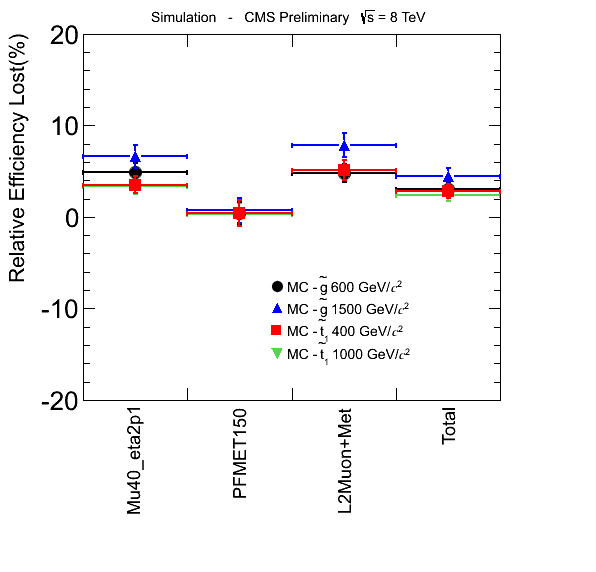
\includegraphics[clip=true, trim=0.0cm 0cm 2.8cm 0cm, width=0.44\textwidth]{figures/syst/syst_8TeVMatchedSAEffLost}
%  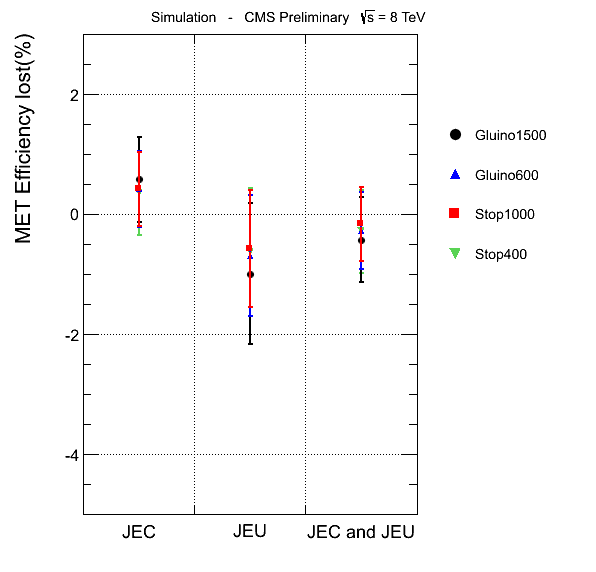
\includegraphics[clip=true, trim=0.0cm 0cm 0cm 0.0cm, width=0.44\textwidth]{figures/syst/summaryEffLossMET55}
%\caption{Relative change in trigger efficiency seen after applying uncertainties for various signals.
%Left: Shifting the synchronization of the muon trigger system as a function of different triggers. The last bin on the X-axis is for the logical OR of the three triggers.
%Right: Adjusting the jet energy scale and recalculating MET. From left to right bins have only JEC applied, only JEU applied, and both JEC and JEU applied.
%    \label{fig:MuSynch}}
%\end{figure}

%Fractionally charged particles have additional systematic uncertainty because their smaller energy depositions mean their hits may not be above thresholds in the muon system
%and tracks will not be found. This simulation of muon system electronics and gas gain can affect this reconstruction efficiency. This was modelled by shifting
%the gain in the muon system by 25\%~\cite{GasGain}. This variation resulted in a signal efficiency change of 15\% (3\%) for $Q = e/3$ ($2e/3$).

Also contributing to the trigger uncertainty is the accuracy of PFMET in the trigger in the MC simulation. The uncertainty on the PFMET is dominated by the uncertainty on
the measurement of jet energies. The jet/MET POG within CMS studies the agreement between data and simulation for jets. For both data and MC simulation,
the group releases corrections to the energy scale of jets (JEC) which can be applied after reconstruction to give the best measurement of the energy of the jet. The corrections
come with corresponding uncertainties (JEU). The jets used for calculating the PFMET at trigger level are not corrected.

To determine the systematic uncertainty, the jets in the signal samples are adjusted by both the JEC and JEU and the MET is recalculated.
The jets are corrected by the MC simulation JEC and then by the inverse of the data JEC.
This results in the MC simulation jets having the same properties as uncorrected jets in data.
The JEU are applied by decreasing the energy of each jet by its uncertainty.
%Figure~\ref{fig:MuSynch} shows the efficiency change when applying the JEC and JEU, both individually and together. 
The JEC are found to increase the efficiency slightly while the JEU decrease it by approximately 1\%.
Conservatively, no scale factor is applied on the trigger efficiency and a 1\% uncertainty is taken on the MET trigger for all samples.

The total systematic uncertainty on trigger efficiency is found by combining the above effects. 
The uncertainty on the muon trigger is completely dominant for all samples except for the charge suppressed samples where the muon trigger does not have any efficiency.
For those samples, the trigger efficiency uncertainty comes only from the MET trigger uncertainty.

%The evaluation of trigger uncertainties requires the creation of new samples which take a large
%amount of time and computing resources to create, making it not feasible to evaluate them for all mass and model points, individually. Instead, the uncertainties were evaluated
%for a few representative points including the samples expected to have the largest effect. Then the remaining signal points were assigned one of the evaluated
%uncertainties, always being conservative and assigning the uncertainty from a signal point which would have a larger effect.

\subsection{Uncertainty on Selection Variables}

The uncertainty on the \invbeta\ measurement is studied using muons from the decay of Z bosons. 
Events must have a pair of oppositely charged muons with an invariant mass of $M_Z \pm 10$~GeV. 
Both muons from the decay are required to pass the tight selection (see Section.~\ref{sec:timingintro}) provided by the muon POG.
Only the two muons forming the combination
are used. If more than one such pair exists, the pair with invariant mass closest to $M_Z$ is used. 
The distribution of \invbeta\ in data and MC is compared using only DT measurements, only CSC measurements, and combining the measurements.
The distributions of data and MC are found to agree well both in mean and width for all of the comparisons.
The largest discrepancy in the averages between data and MC is found to be 0.005 and this is taken as the uncertainty on the \invbeta\ measurement.
The effect of this uncertainty on the total signal efficiency is evaluated by shifting the measured \invbeta\ value for signal MC down by 0.005.
This results in an efficiency change of less than 7\% for all considered signals.

The uncertainties on the $p_T$ measurement from the stand-alone and tracker track are determined by
varying the $1/p_T$ values by prescriptions from the muon POG~\cite{2012JInst...7P0002T}. For the \muononly\
analysis, the $1/p_T$ of the stand-alone track is shifted up by 10\%, this means that the \pt\ will decrease.
For the other analyses the $1/p_T$ of the inner track is adjusted by the Equation

\begin{equation}
 \frac{1}{p_T\prime} = \frac{1}{p_T} + \delta_{K_T}(q, \phi, \eta)
\end{equation}

\begin{equation}
 \delta_{K_T}(q, \phi, \eta) = A + B\eta^2 + qC\sin(\phi - \phi_0)
\end{equation}
where A = 0.236 TeV$^{-1}$, B = -0.135 TeV$^{-1}$,
C = 0.282 TeV$^{-1}$, and $\phi_0$ = 1.337. The shifts were found to have a less than 10\% effect on the efficiency to pass the final selection for all signals.

The effect of the uncertainty on \dedx\ was evaluated with low momentum protons. Protons with $p$ less than  about 2~GeV will have speed appreciably lower than the
speed of light and thus will appear similar to signal particles. A comparison of data and simulation yields an uncertainty of 0.05 on \ias\ and 5\% on \ih. %These uncertainties,
When propagated to the final selection for singly charged particles, these uncertainties give efficiency changes of less than 13\% for low mass samples
and less than 7\% for masses above 200~GeV/$c^2$. Multiply charged particles have sufficient
separation between signal and background that the uncertainty is negligible.

%For fractionally charged particles the uncertainty on \dedx\ also affects the track reconstruction efficiency as if the energy is too low the hits will not be reconstructed.
%To evaluate this 

\subsection{Other Uncertainties on Signal Efficiency}

The systematic uncertainty on the efficiency to reconstruct muons~\cite{2012JInst...7P0002T} and tracks~\cite{CMS:2010mua} were both found to be less than 2\%.
Additionally for the \muononly\ analysis, a 1\% uncertainty recommended by the muon POG is applied on the correction factors described in Section~\ref{sec:TagProbe}.

The uncertainty on the number of proton-proton collisions per bunch crossing is found by varying by 6\% the 
proton-proton cross-section used to determine the weights for MC simulation events (see end of Sec.~\ref{sec:samples}).
This leads to an uncertainty of less than 4\% for all samples.

Multiply charged particles deposit a large amount of energy in the calorimeter and if the particle does not have enough energy it may come to a stop in the calorimeter.
This is particularly important for high charge, low mass samples, because if the particle has enough energy to pass through the calorimeter then it will
be traveling at a high speed and be unlikely to pass the threshold on \invbeta. Uncertainty on the amount of detector material, determined mostly by the
HCAL, affects the number of HSCP that will stop. There is a conservative 5\% uncertainty on the material budget as measured by energy loss of cosmic ray muons
passing through CMS~\cite{Chatrchyan:2009si}. Shifting the material density by this amount for a few signal samples has at most a 20\% effect
for the lowest mass, highest $Q$ samples. This 20\% uncertainty is conservatively taken for all multiply charged samples.

\subsection{Total Signal Efficiency Uncertainty}

The total systematic uncertainty for each signal point is found by adding the above effects in quadrature.
Figure~\ref{fig:MuOnlyUncSource} shows the different sources of signal efficiency systematic uncertainty and their quadratic sum
for the various signal models considered in the \muononly\ analysis. The error bars are only statistical.
Figure~\ref{fig:TkMuStauUncSource} and~\ref{fig:TkMuRHadUncSource} shows the same for the \tktof\ analysis for stau and $R-hadron$ models, respectively.
Figure~\ref{fig:TkOnMCUncSource} shows the sources of systematic uncertainty for a few of the samples in the \tkonly\ and \multi\ analyses.

\begin{figure}[ht]
\centering
  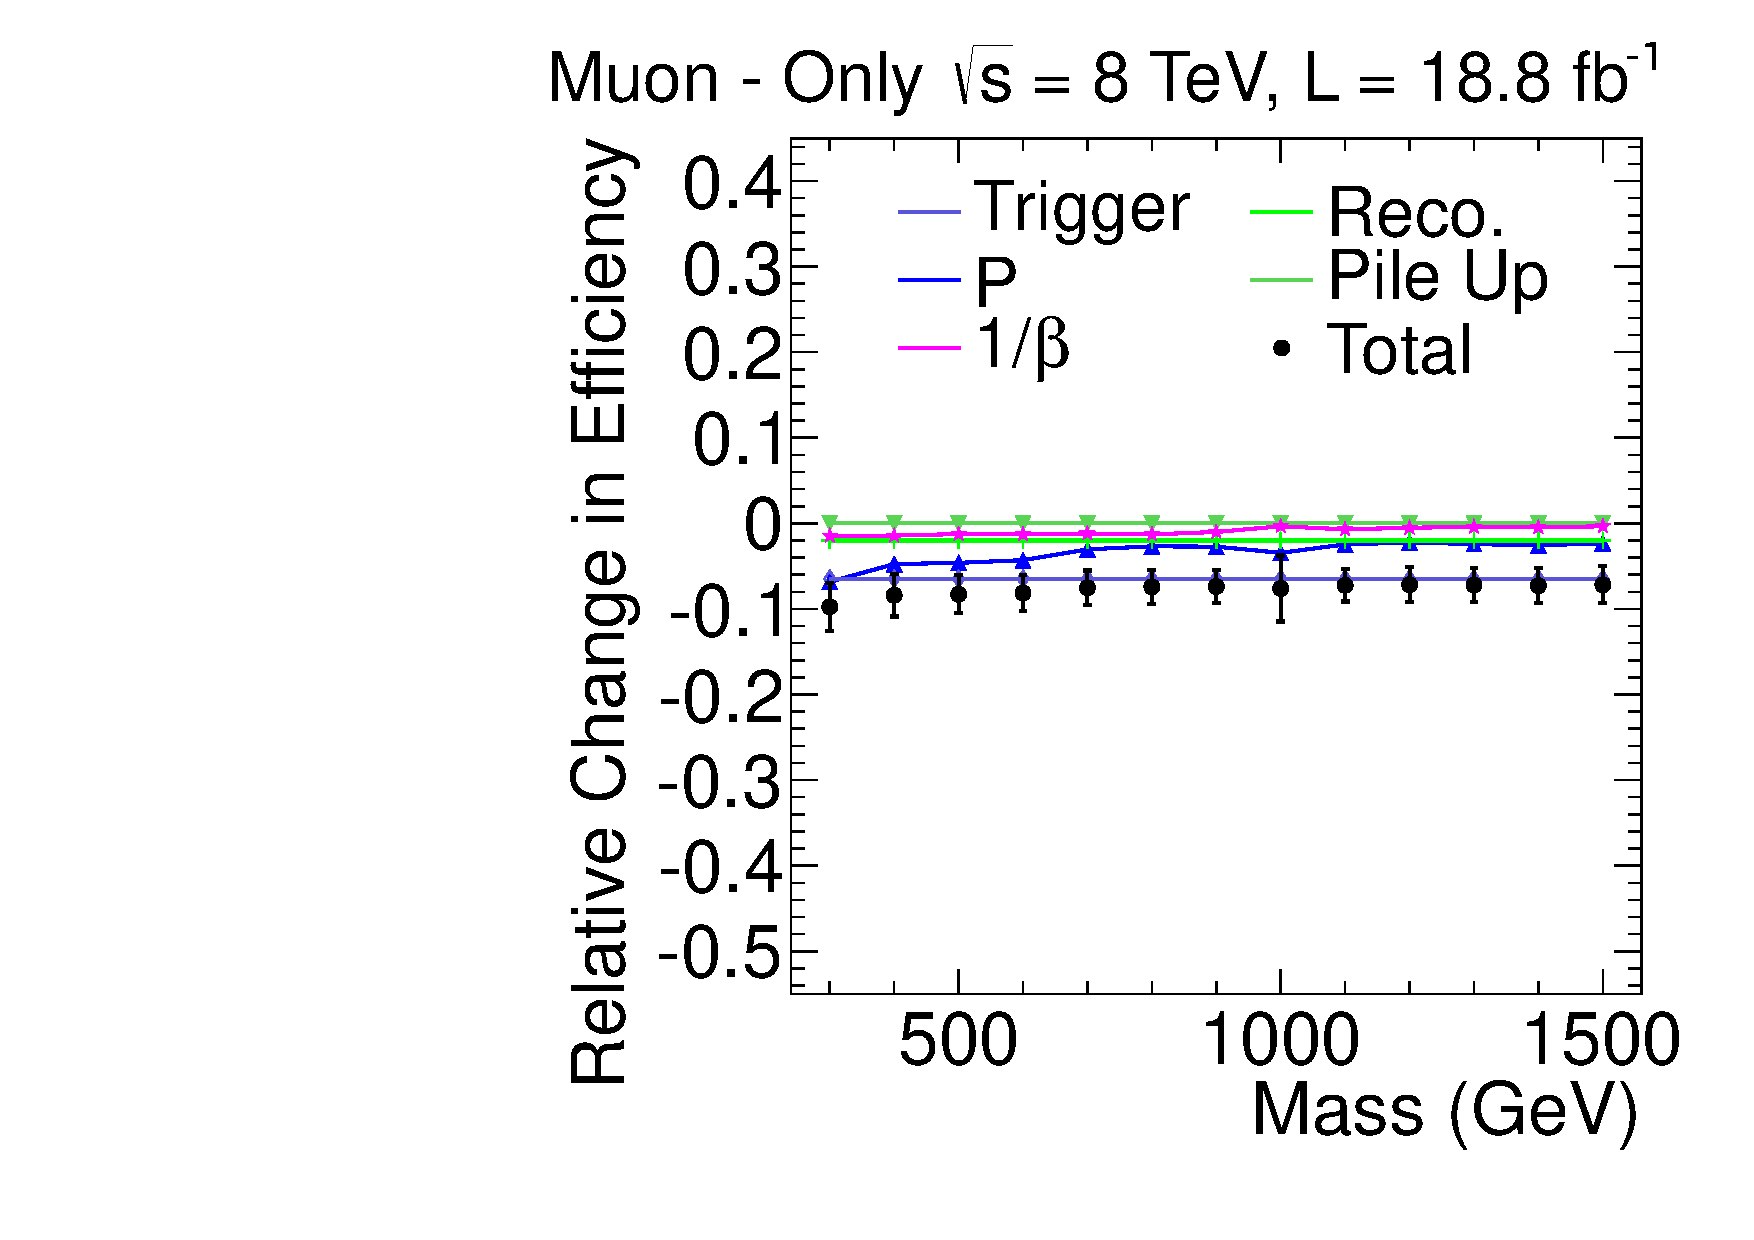
\includegraphics[clip=false, trim=0.0cm 0cm 0.0cm 0cm, width=0.48\textwidth]{figures/muonly/MoGluino_f100Uncertainty}
  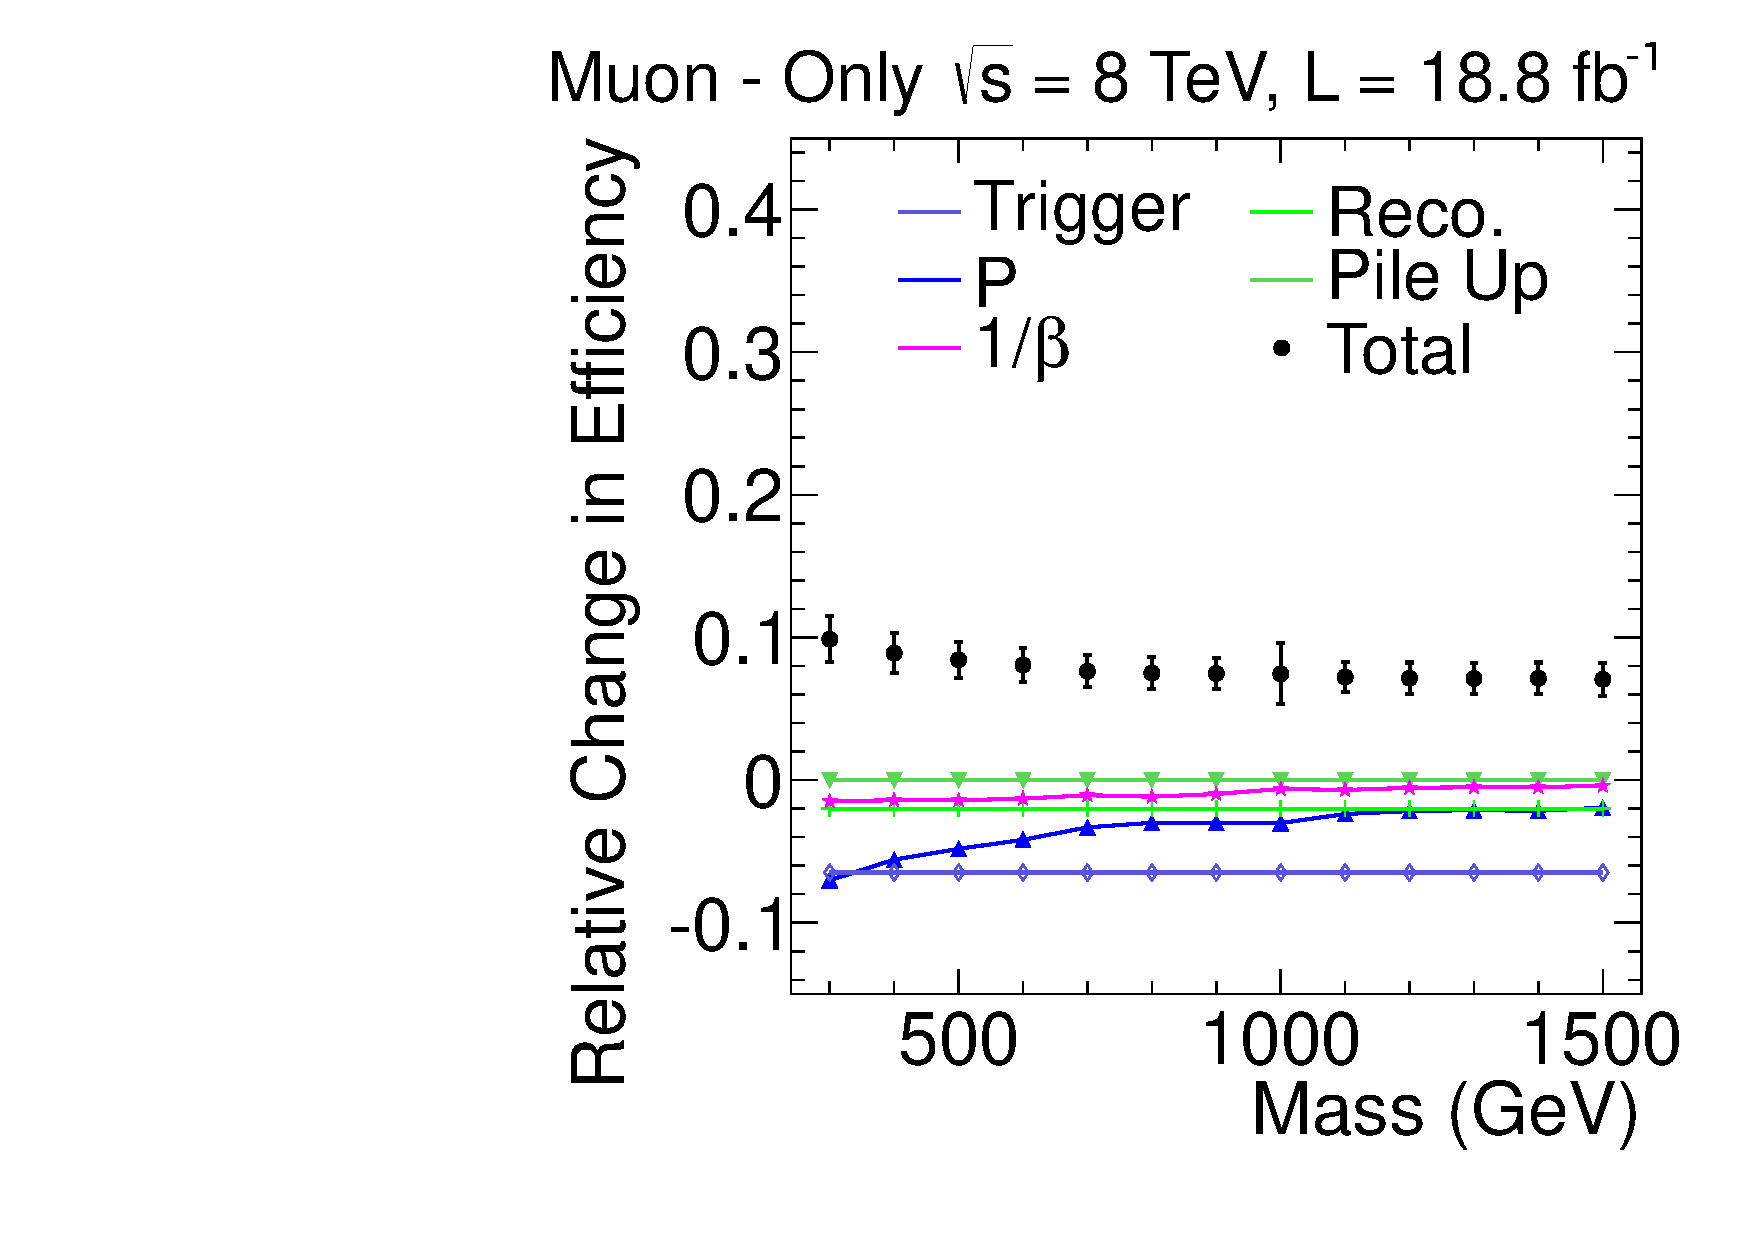
\includegraphics[clip=false, trim=0.0cm 0cm 0.0cm 0cm, width=0.48\textwidth]{figures/muonly/MoGluino_f50Uncertainty} \\
  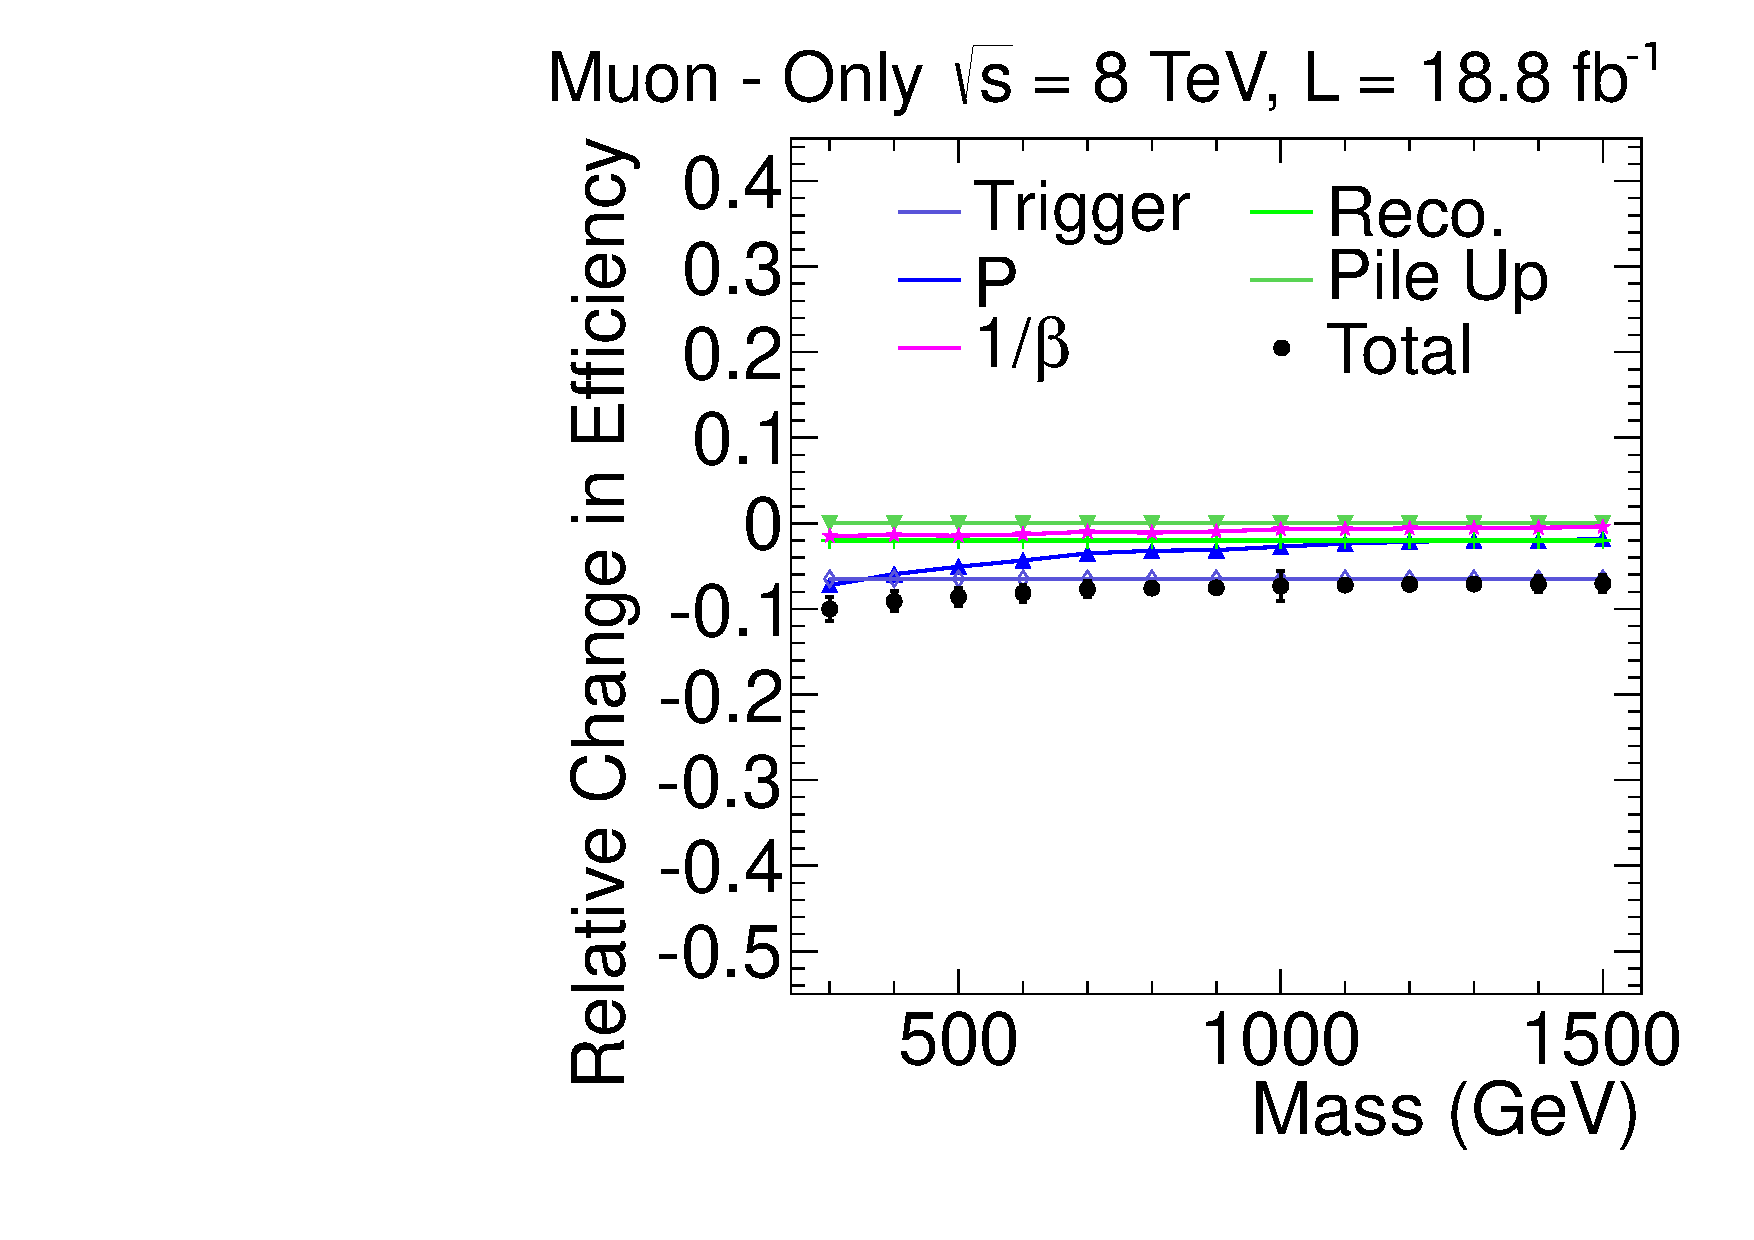
\includegraphics[clip=false, trim=0.0cm 0cm 0.0cm 0cm, width=0.48\textwidth]{figures/muonly/MoGluino_f10Uncertainty}
  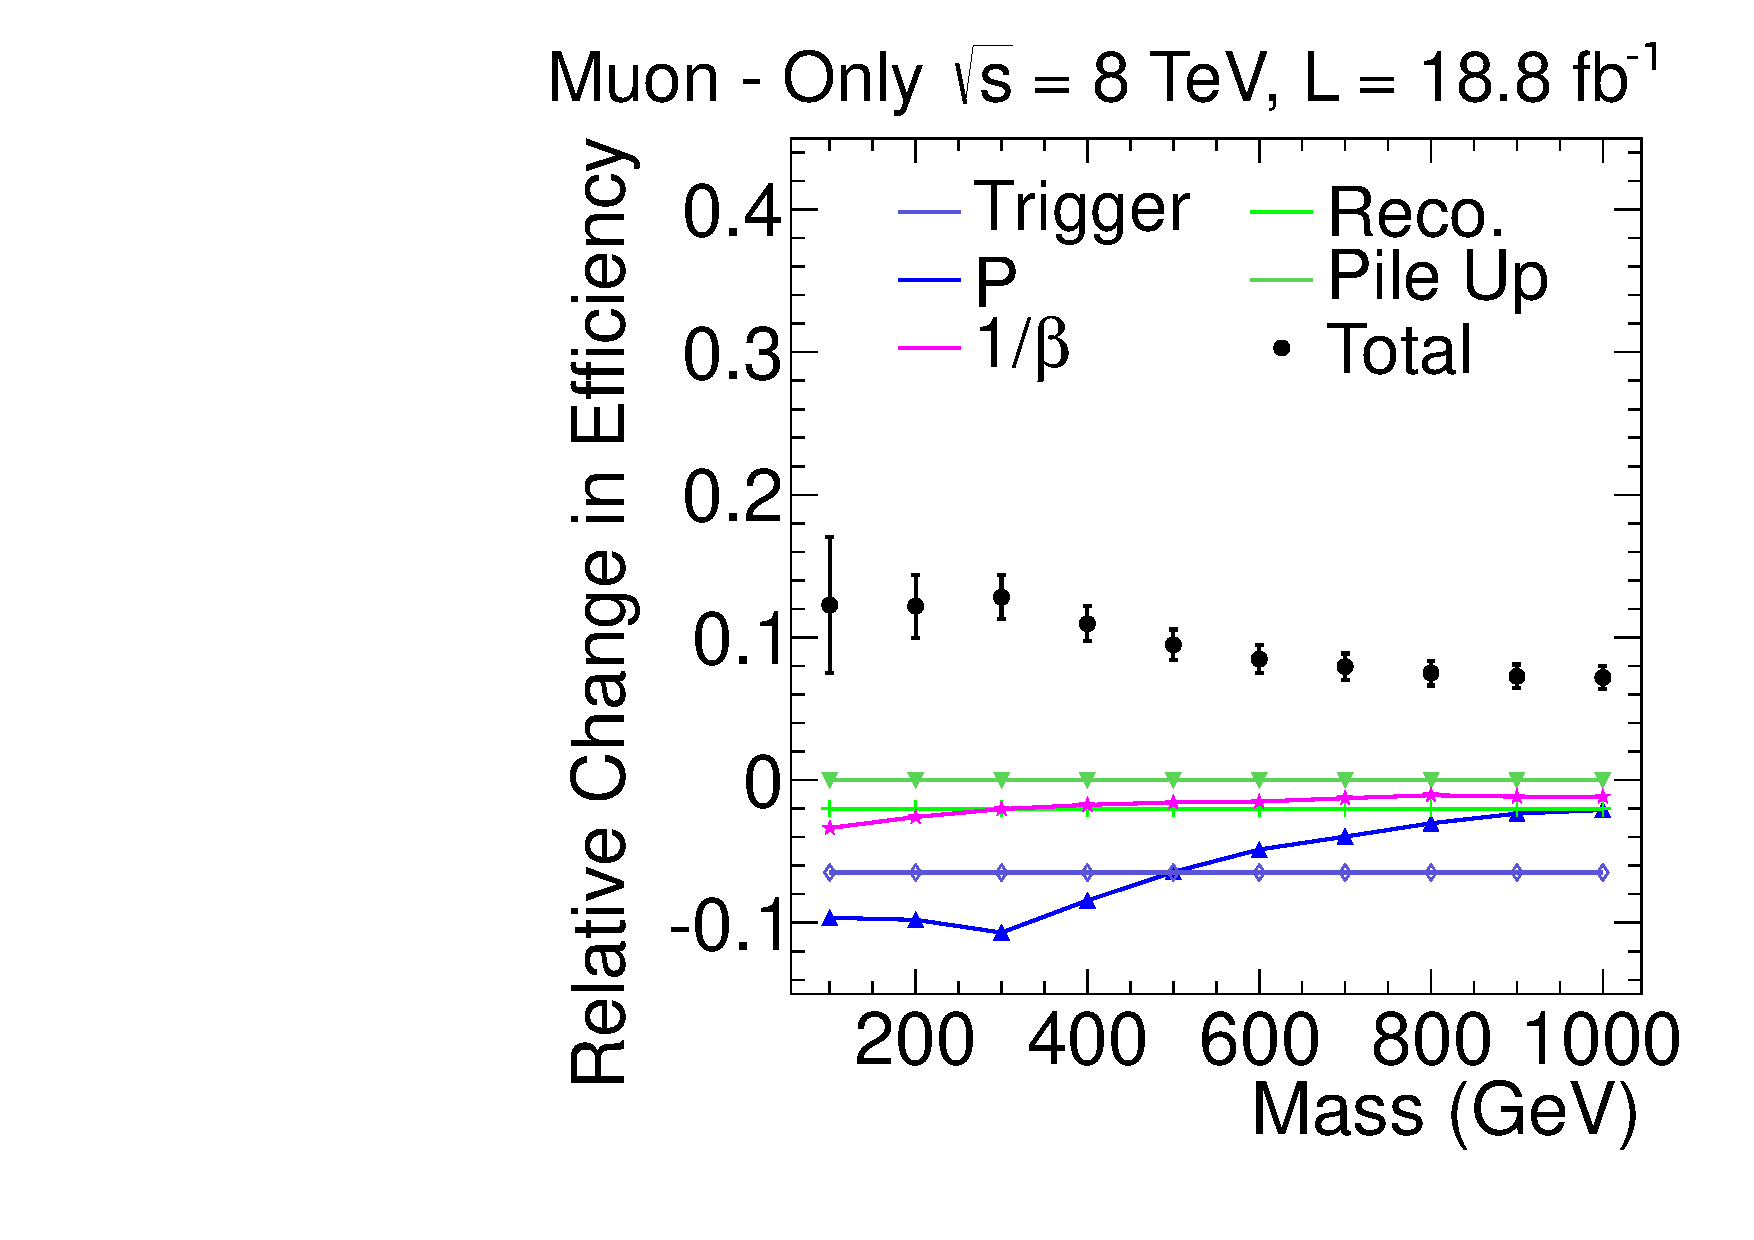
\includegraphics[clip=false, trim=0.0cm 0cm 0.0cm 0cm, width=0.48\textwidth]{figures/muonly/MoStopUncertainty}
\caption[Relative signal efficiency change seen for the various sources of uncertainty in the \muononly\ analysis]
{Relative signal efficiency change seen for the various sources of uncertainty in the \muononly\ analysis.
Error bars show only the statistical uncertainty.
Top row: Gluino with $f=1.0$ (left) and $f=0.5$ (right).
Bottom row: Gluino with $f=0.1$ (left) and stop (right)}
    \label{fig:MuOnlyUncSource}
\end{figure}

\begin{figure}[ht]
\centering
  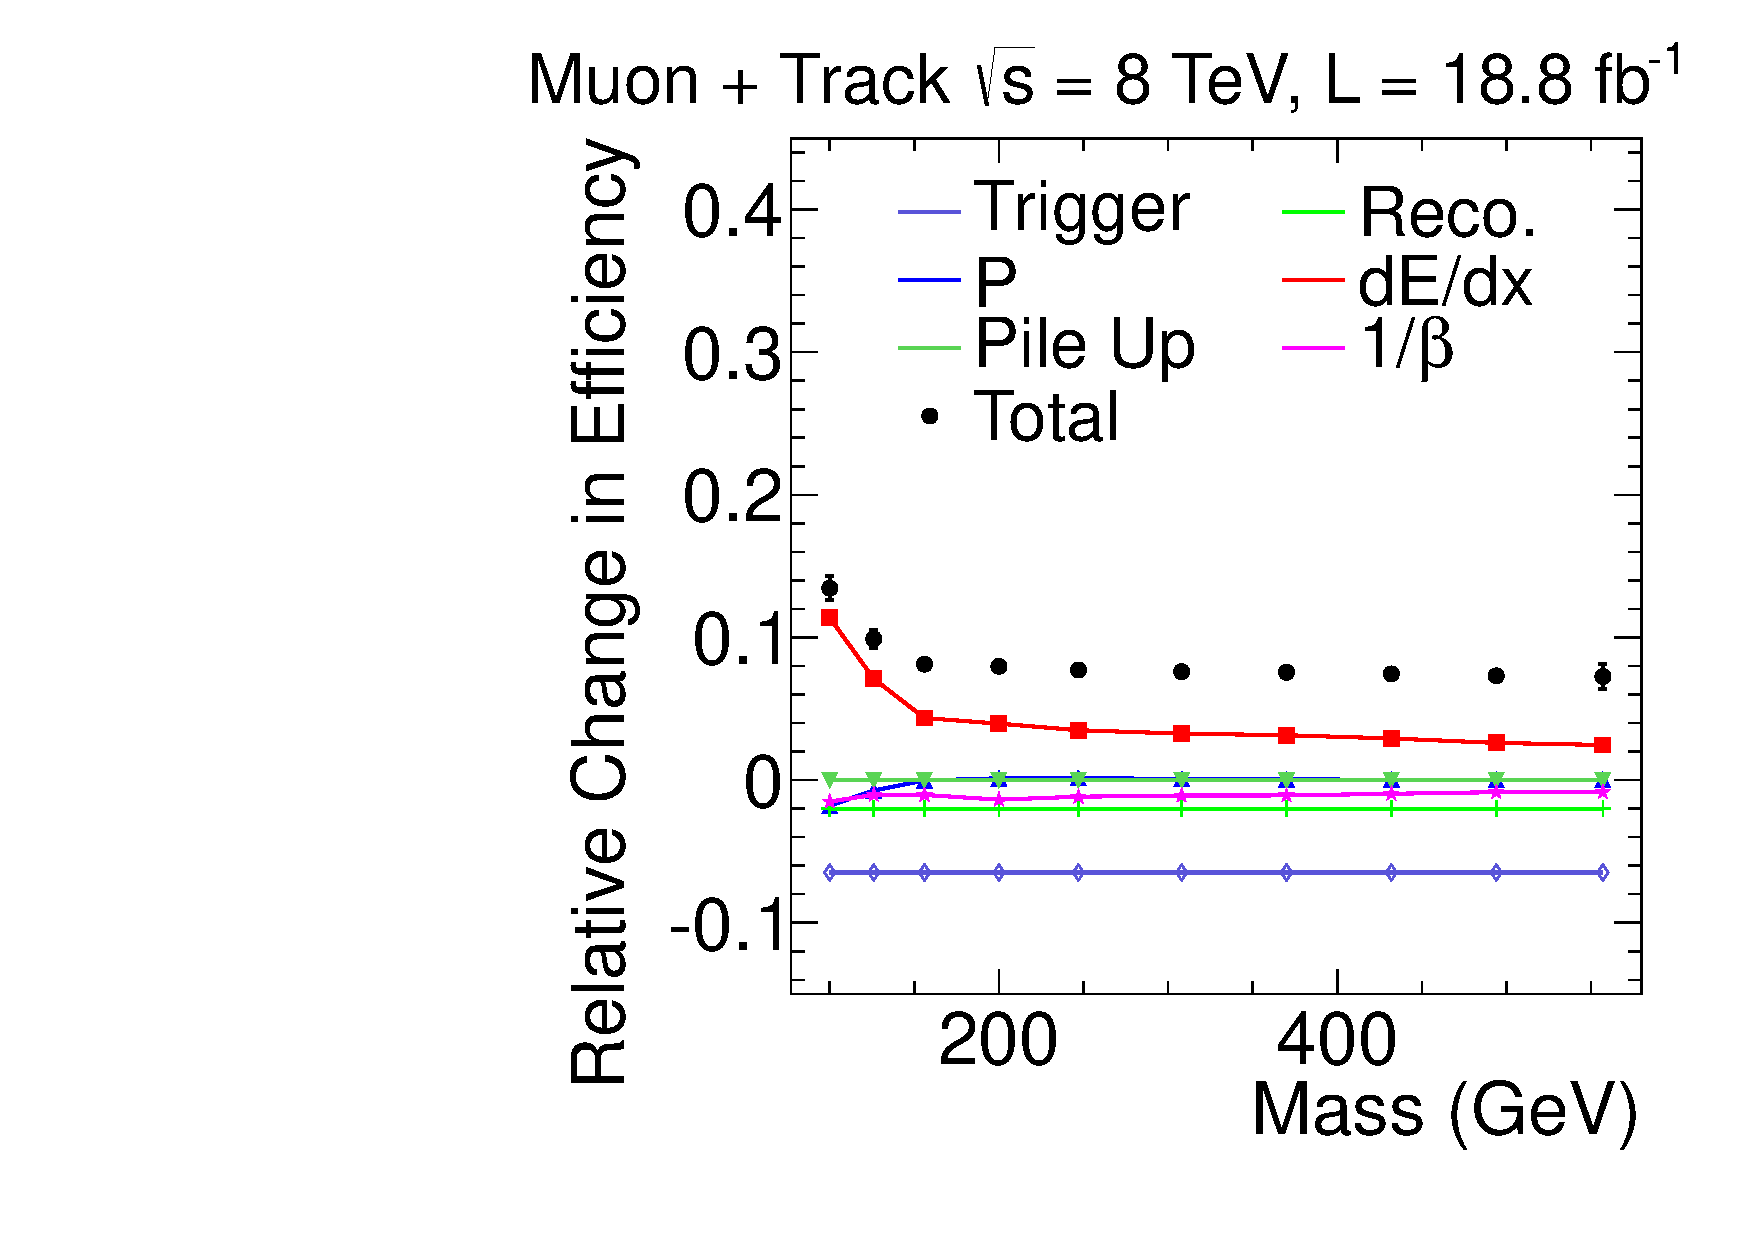
\includegraphics[clip=false, trim=0.0cm 0cm 0.0cm 0cm, width=0.48\textwidth]{figures/tkmu/MuGMStauUncertainty}
  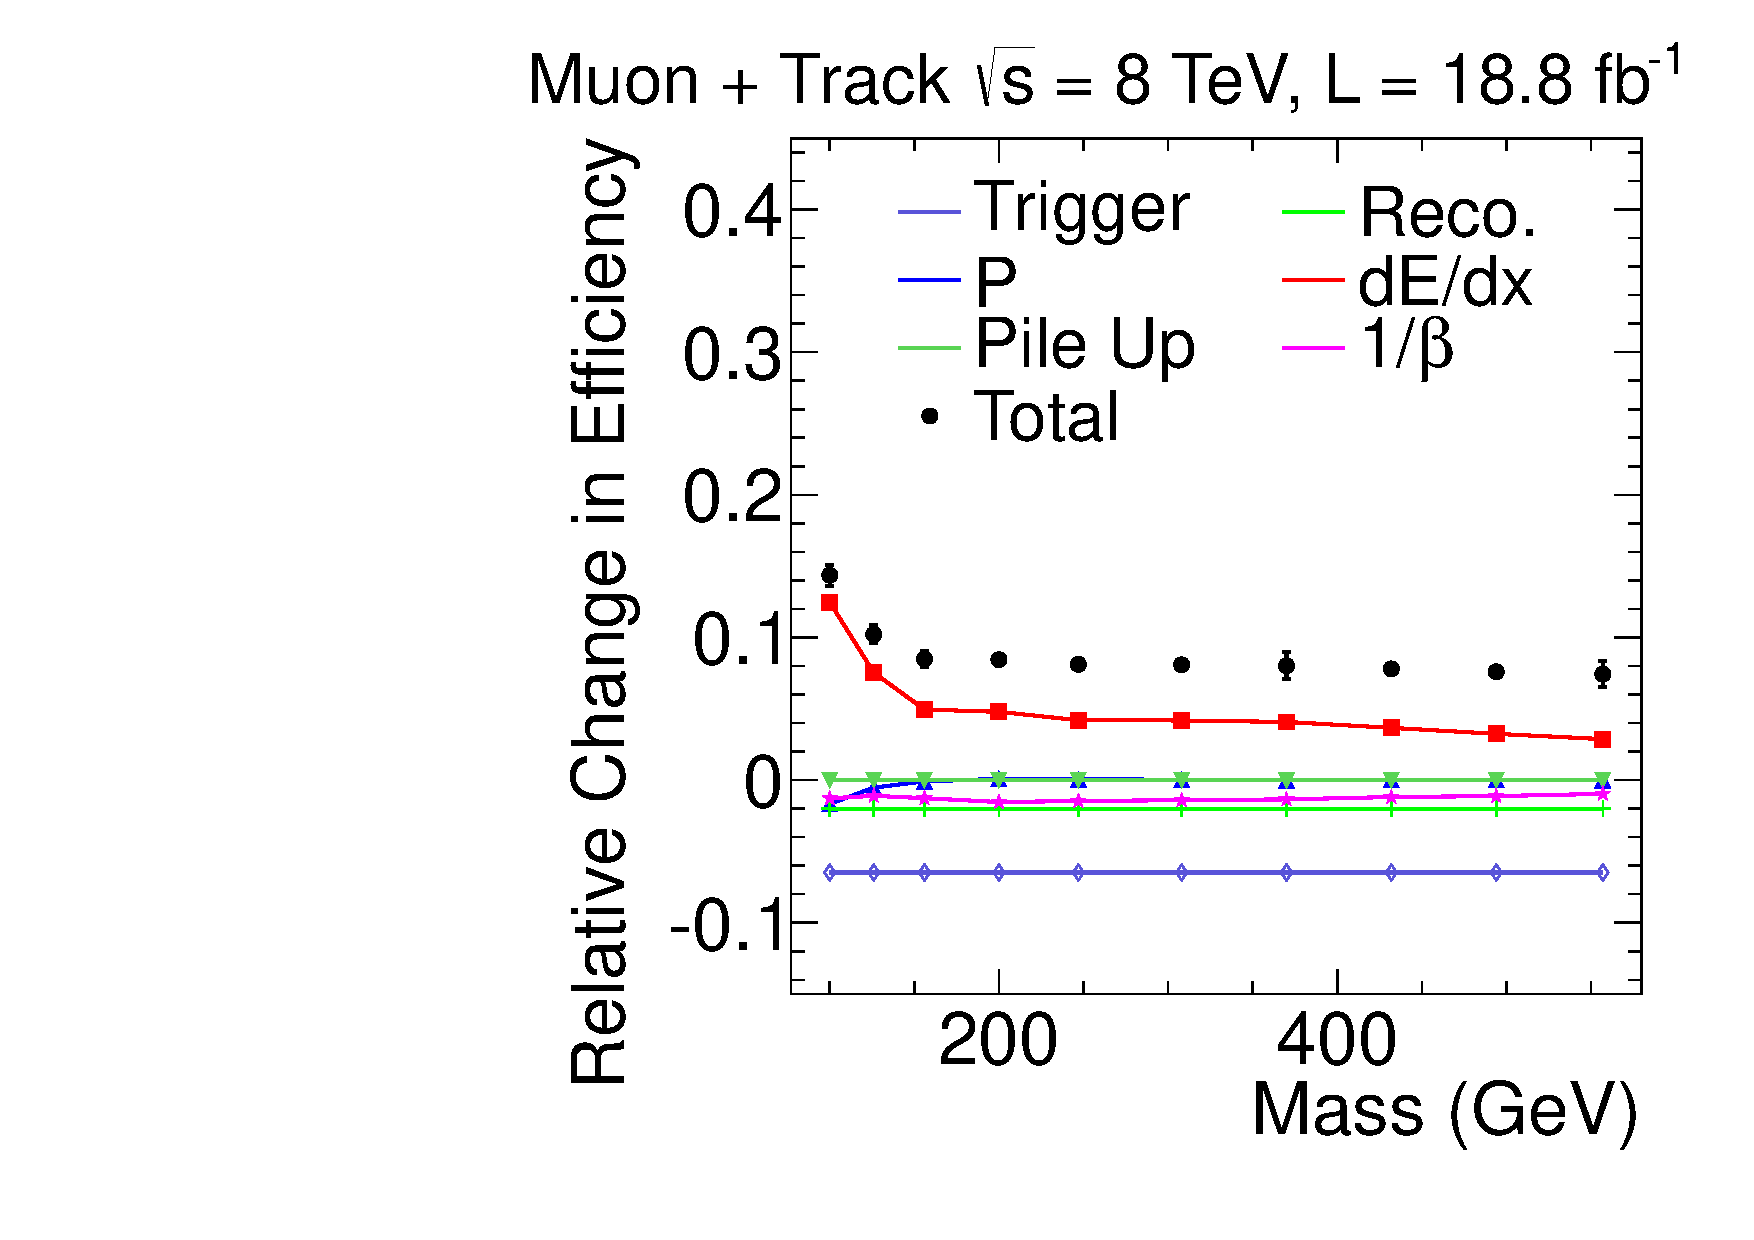
\includegraphics[clip=false, trim=0.0cm 0cm 0.0cm 0cm, width=0.48\textwidth]{figures/tkmu/MuPPStauUncertainty} \\
\caption[Relative signal efficiency change seen for the various sources of uncertainty for stau models in the \tktof\ analysis]
{Relative signal efficiency change seen for the various sources of uncertainty for stau models in the \tktof\ analysis: CD (left) and DP (right).
Error bars show only the statistical uncertainty.
}
    \label{fig:TkMuStauUncSource}
\end{figure}

\begin{figure}[ht]
\centering
  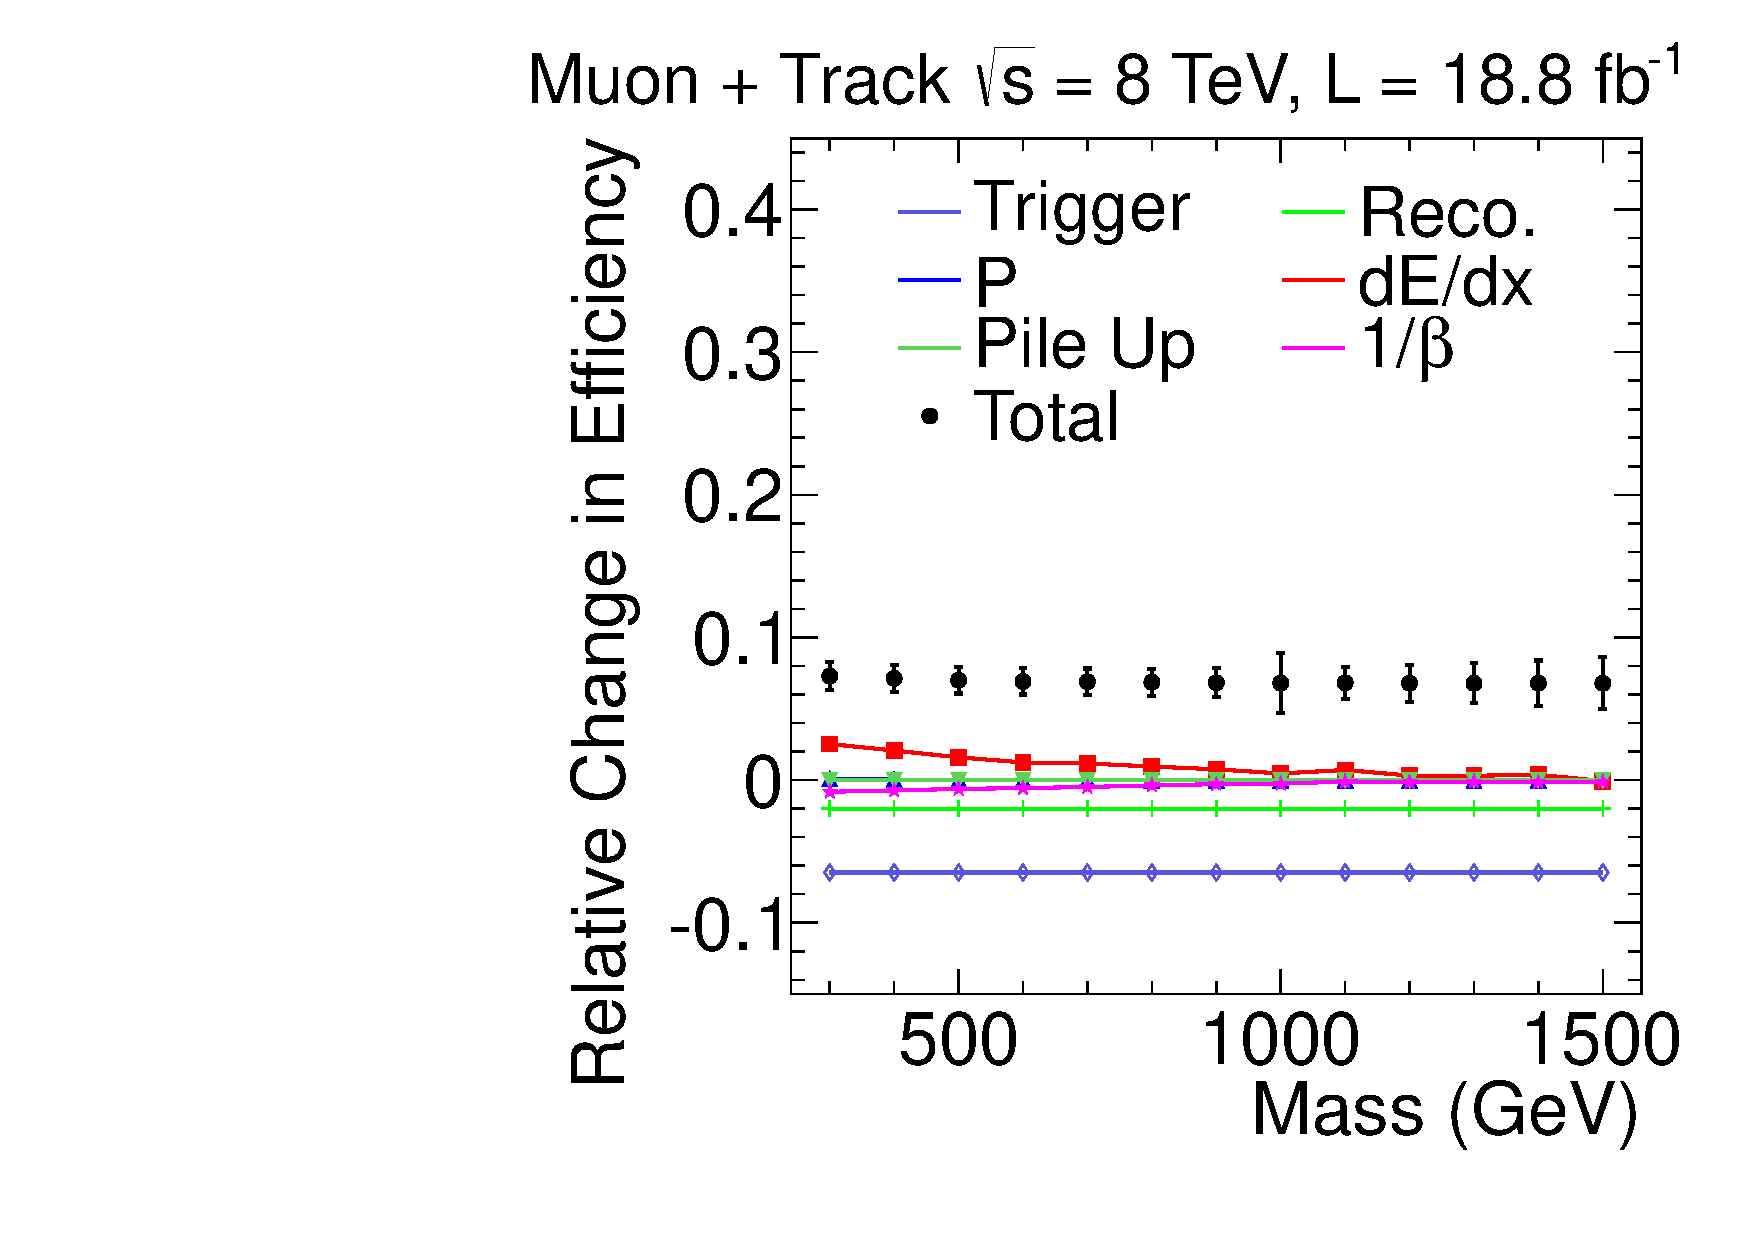
\includegraphics[clip=false, trim=0.0cm 0cm 0.0cm 0cm, width=0.48\textwidth]{figures/tkmu/MuGluino_f50Uncertainty}
  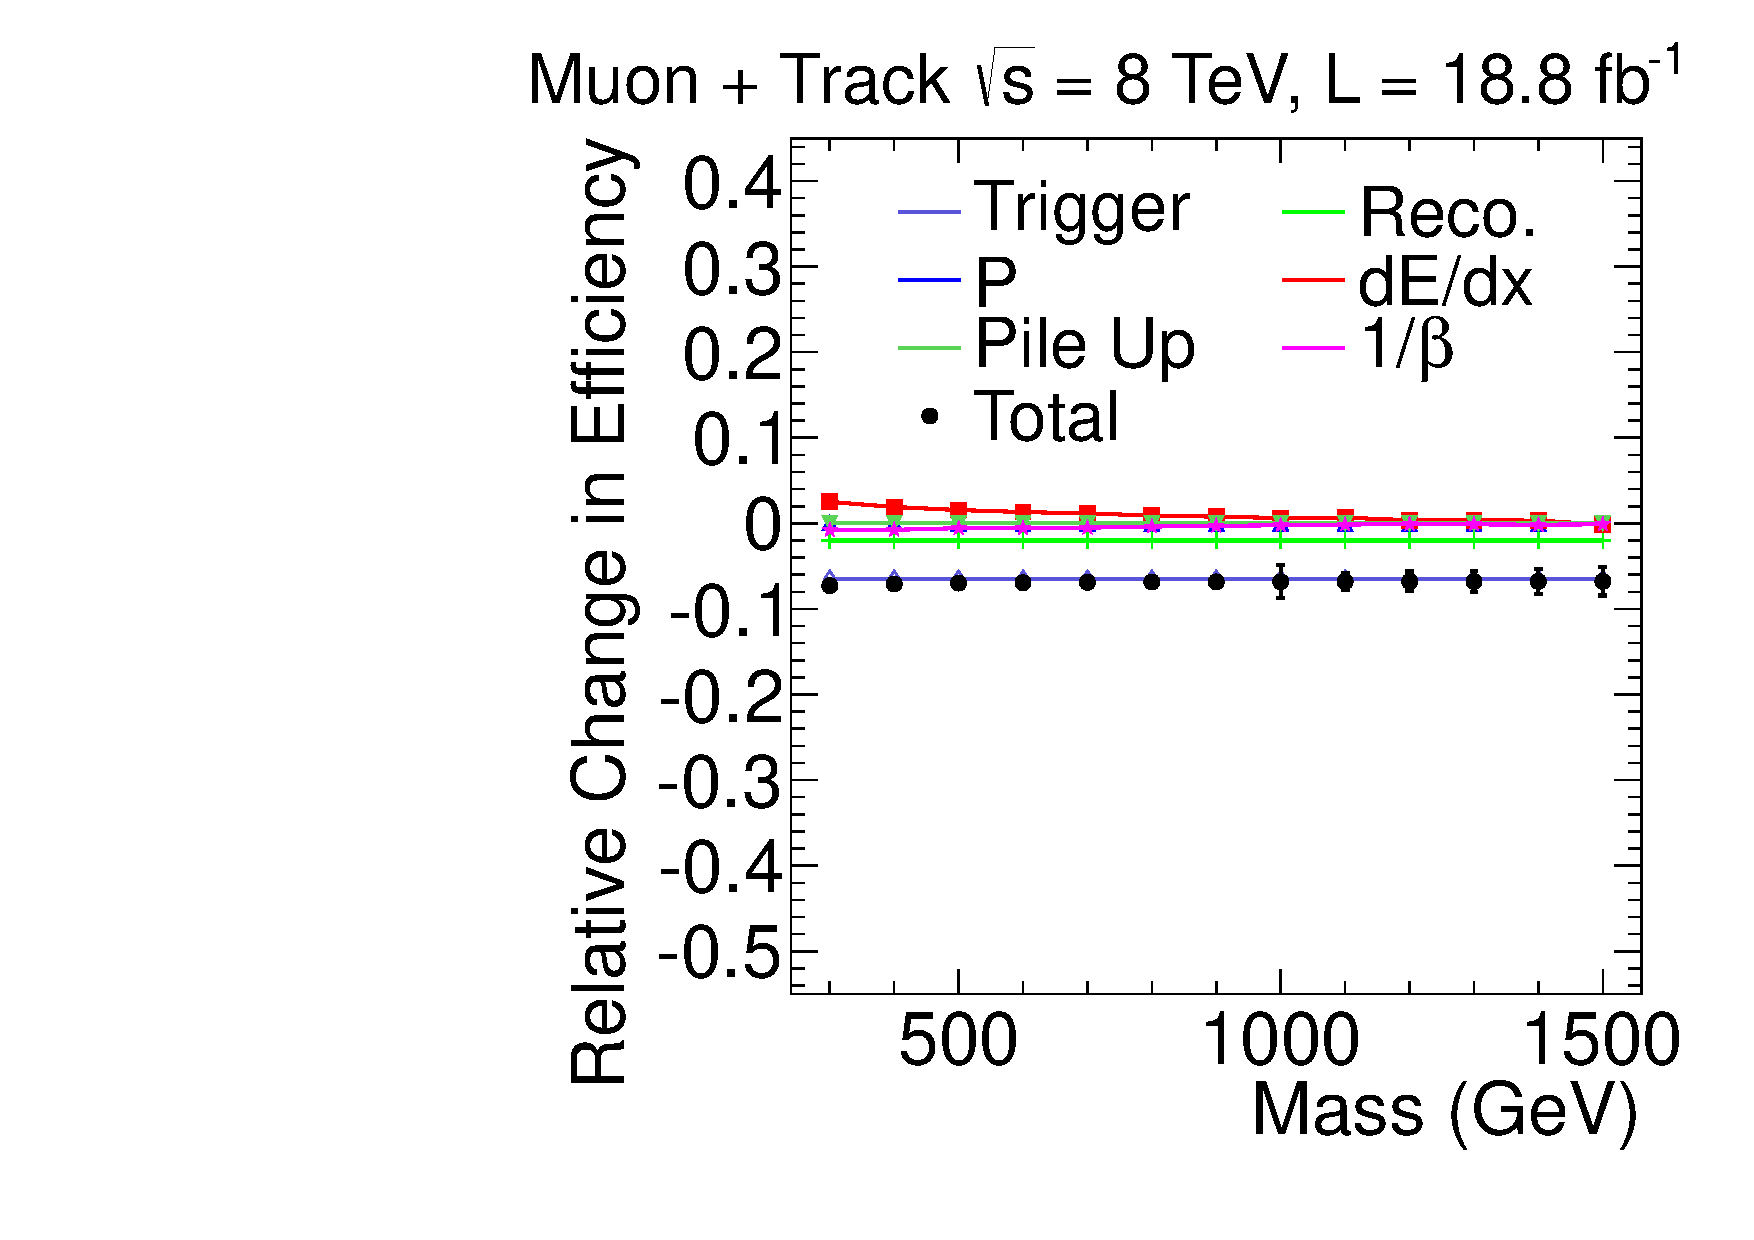
\includegraphics[clip=false, trim=0.0cm 0cm 0.0cm 0cm, width=0.48\textwidth]{figures/tkmu/MuGluino_f10Uncertainty}\\
  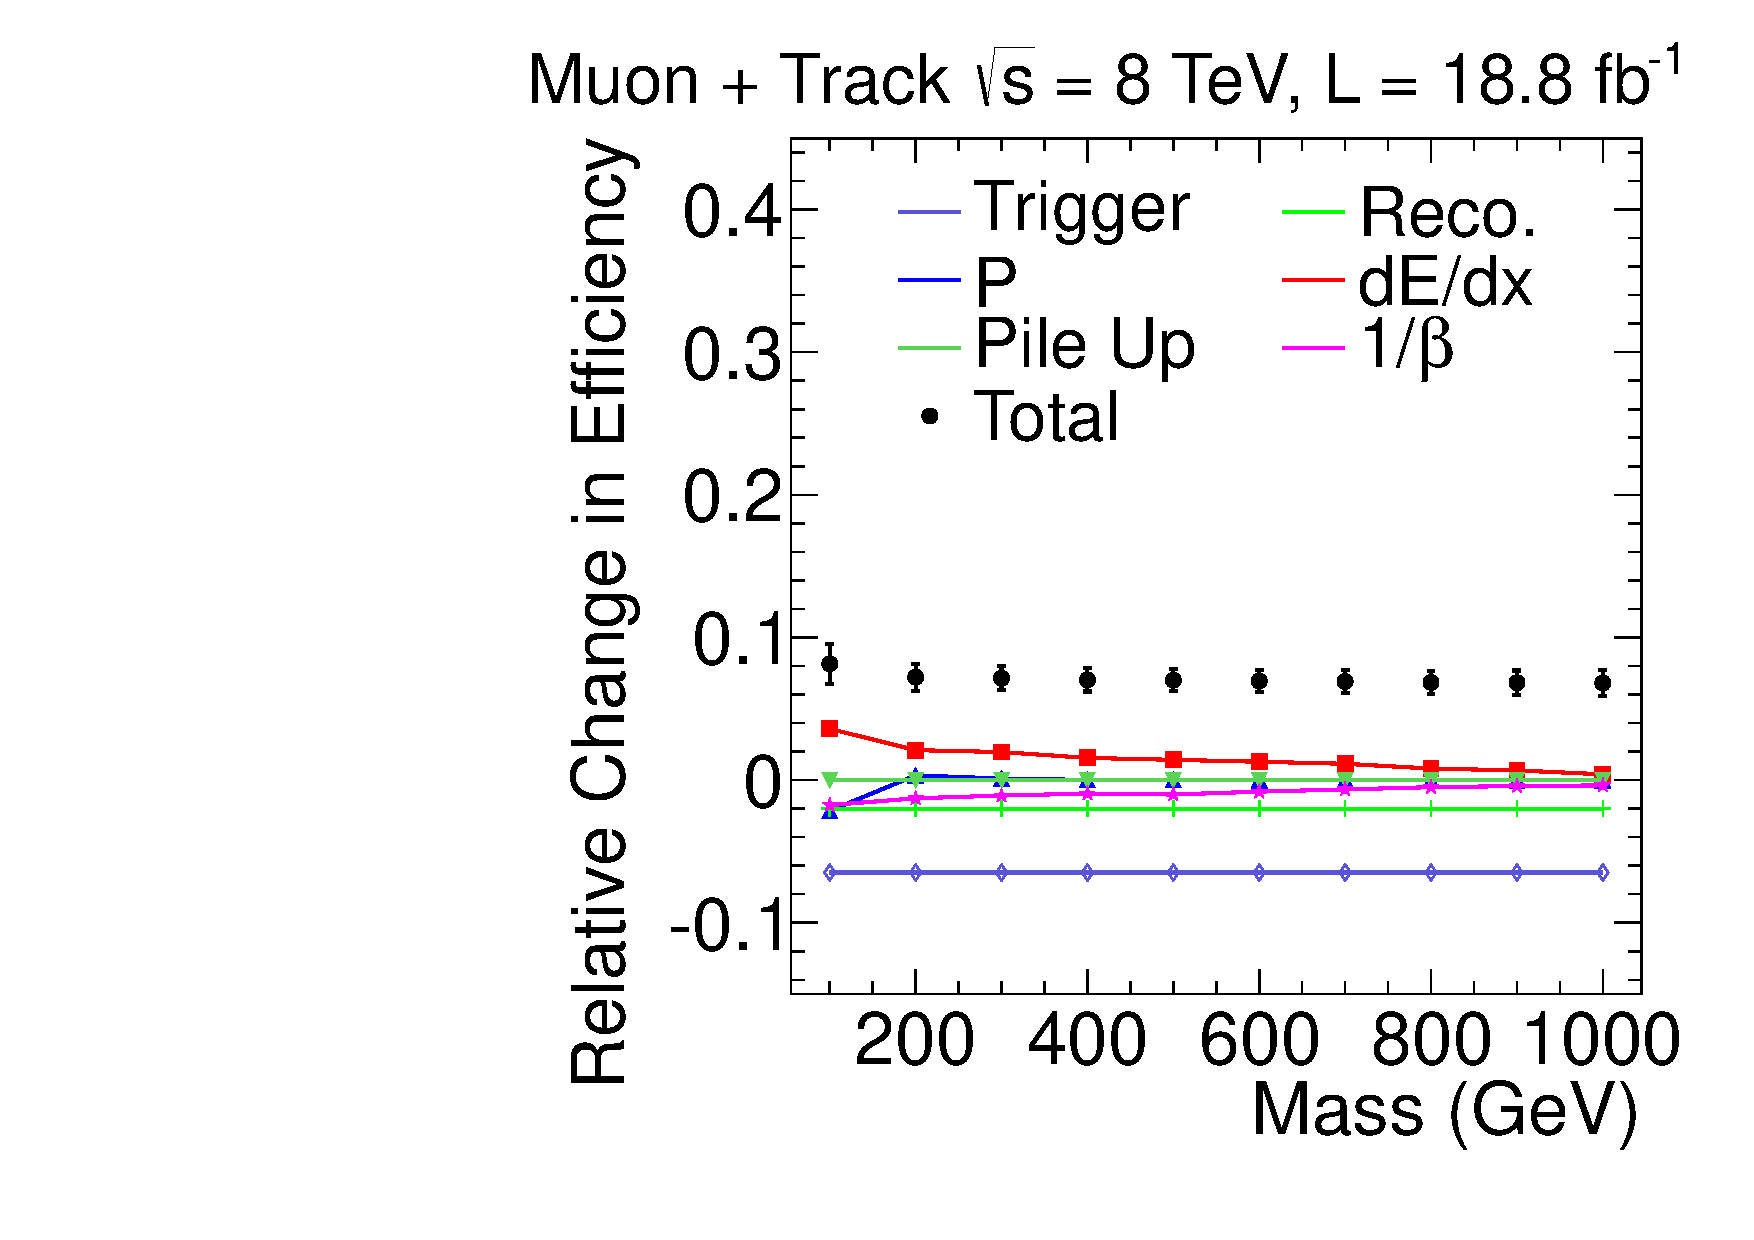
\includegraphics[clip=false, trim=0.0cm 0cm 0.0cm 0cm, width=0.48\textwidth]{figures/tkmu/MuStopUncertainty}
\caption[Relative efficiency change seen for the various sources of uncertainty for $R-hadron$ models in the \tktof\ analysis]
{Relative efficiency change seen for the various sources of uncertainty for $R-hadron$ models in the \tktof\ analysis.
Error bars show only the statistical uncertainty.
Top row: Gluino with $f=0.5$ (left) and $f=0.1$ (right).
Bottom row: Stop}
    \label{fig:TkMuRHadUncSource}
\end{figure}

\begin{figure}[ht]
\centering
  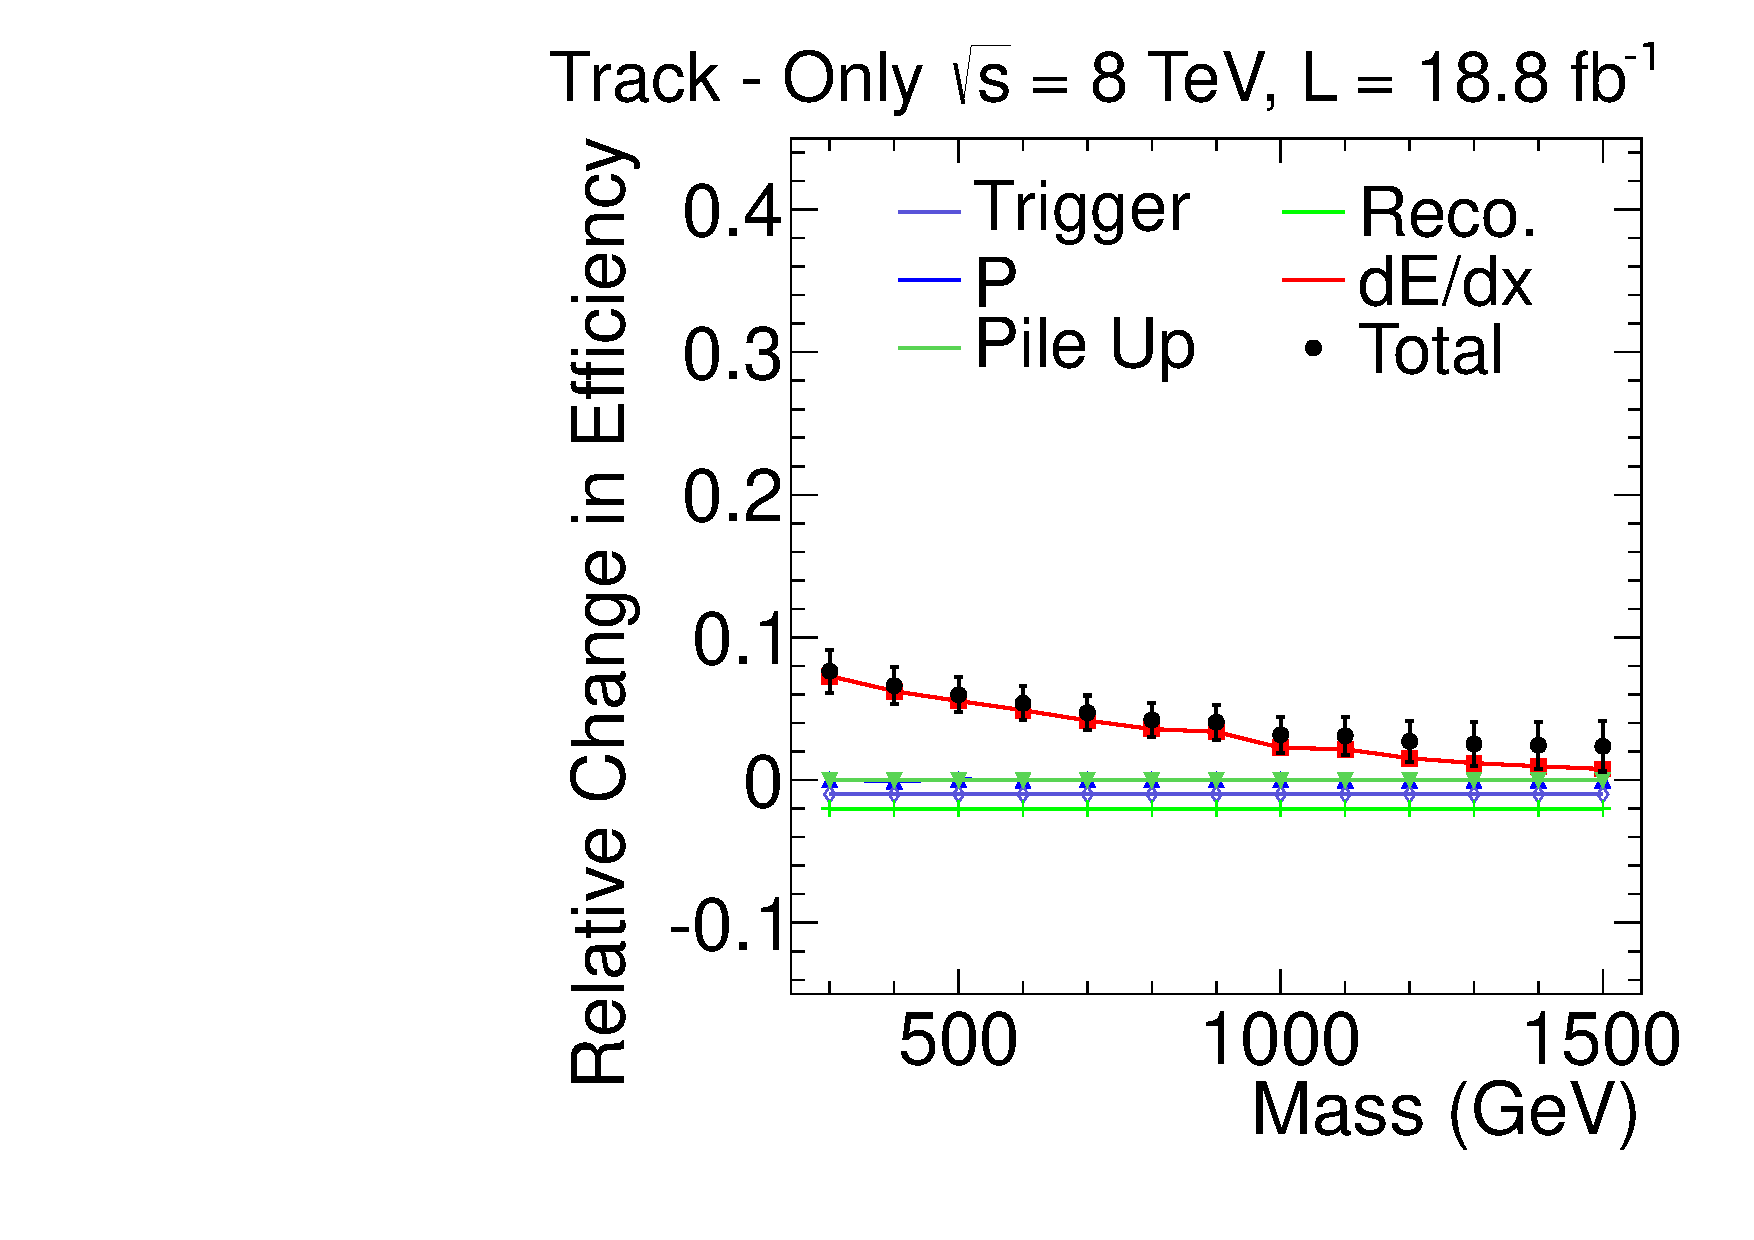
\includegraphics[clip=false, trim=0.0cm 0cm 0.0cm 0cm, width=0.48\textwidth]{figures/tkonly/TkGluinoN_f10Uncertainty}
  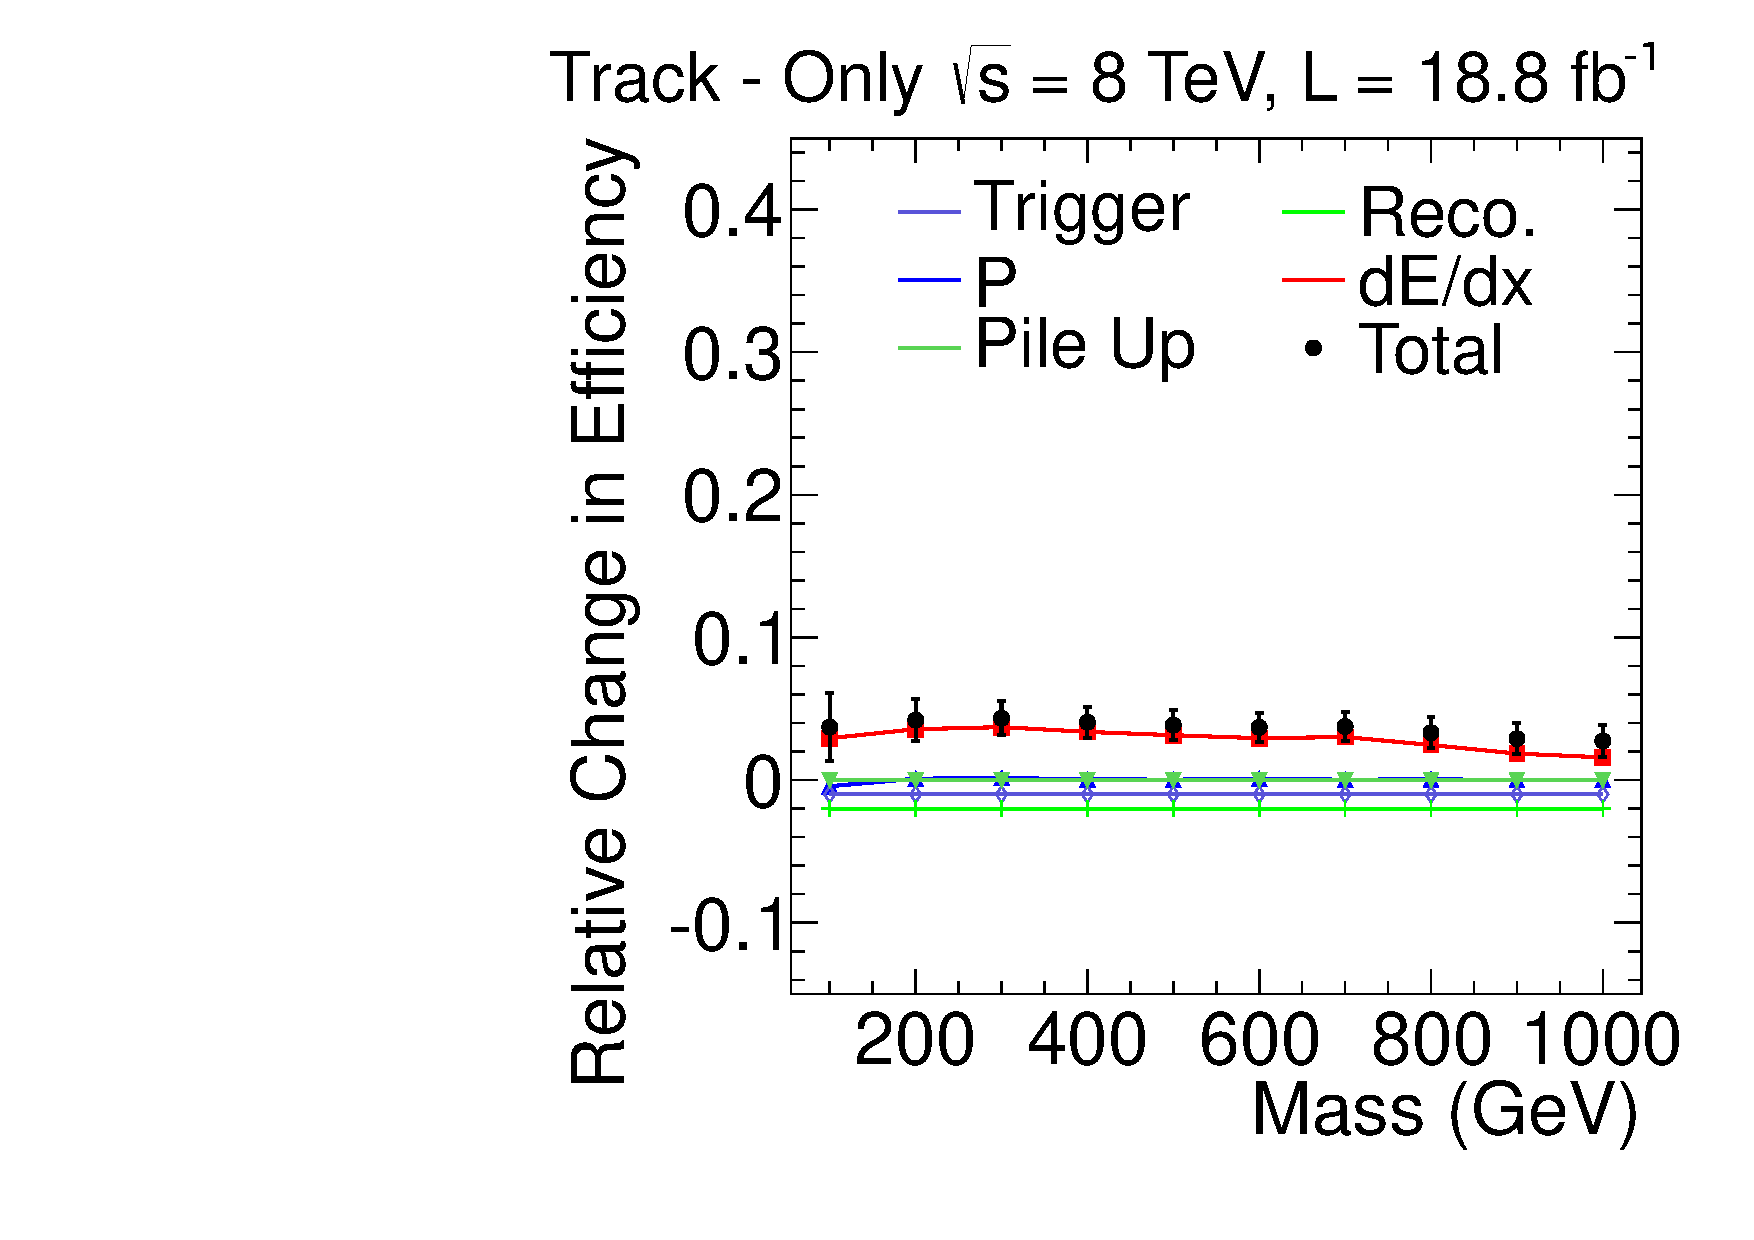
\includegraphics[clip=false, trim=0.0cm 0cm 0.0cm 0cm, width=0.48\textwidth]{figures/tkonly/TkStopNUncertainty}\\
  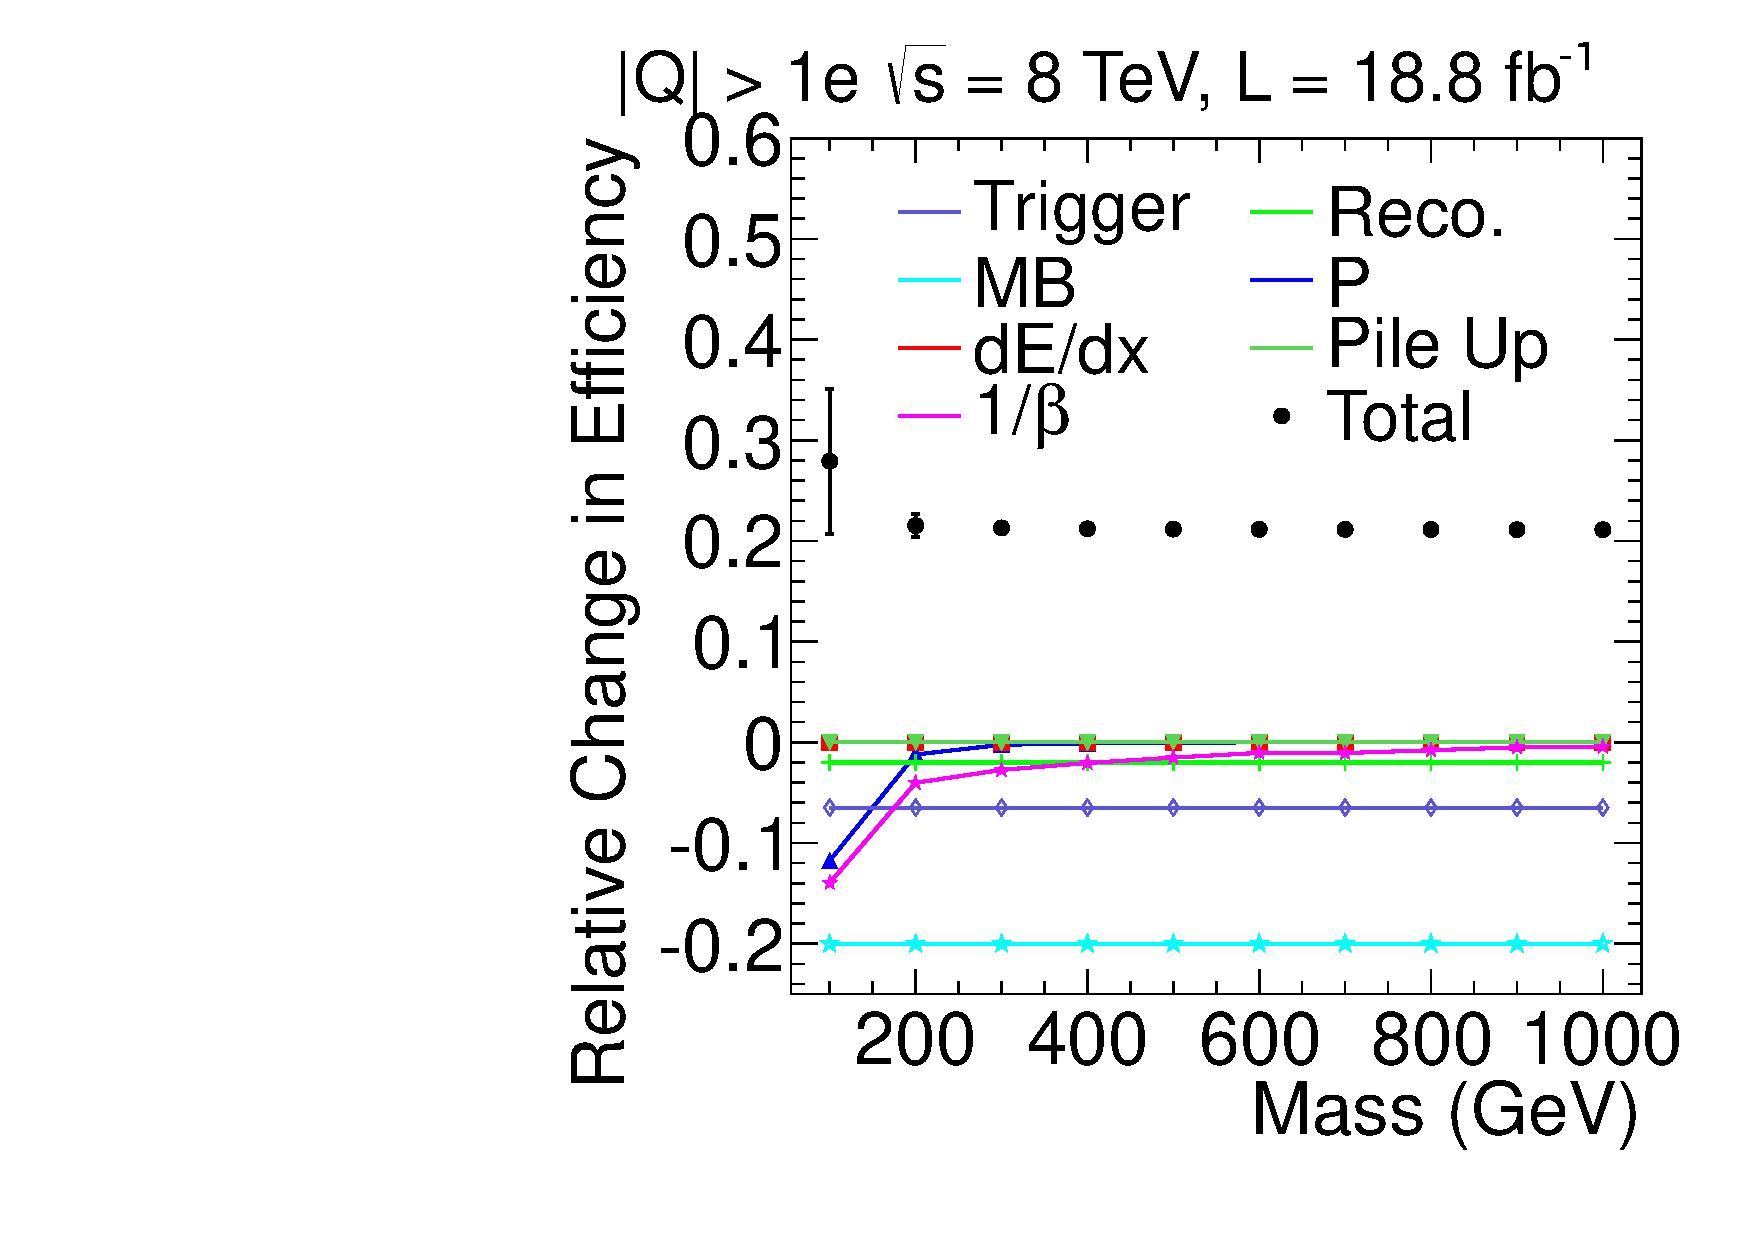
\includegraphics[clip=false, trim=0.0cm 0cm 0.0cm 0cm, width=0.48\textwidth]{figures/multi/HQDY_Q4Uncertainty}
  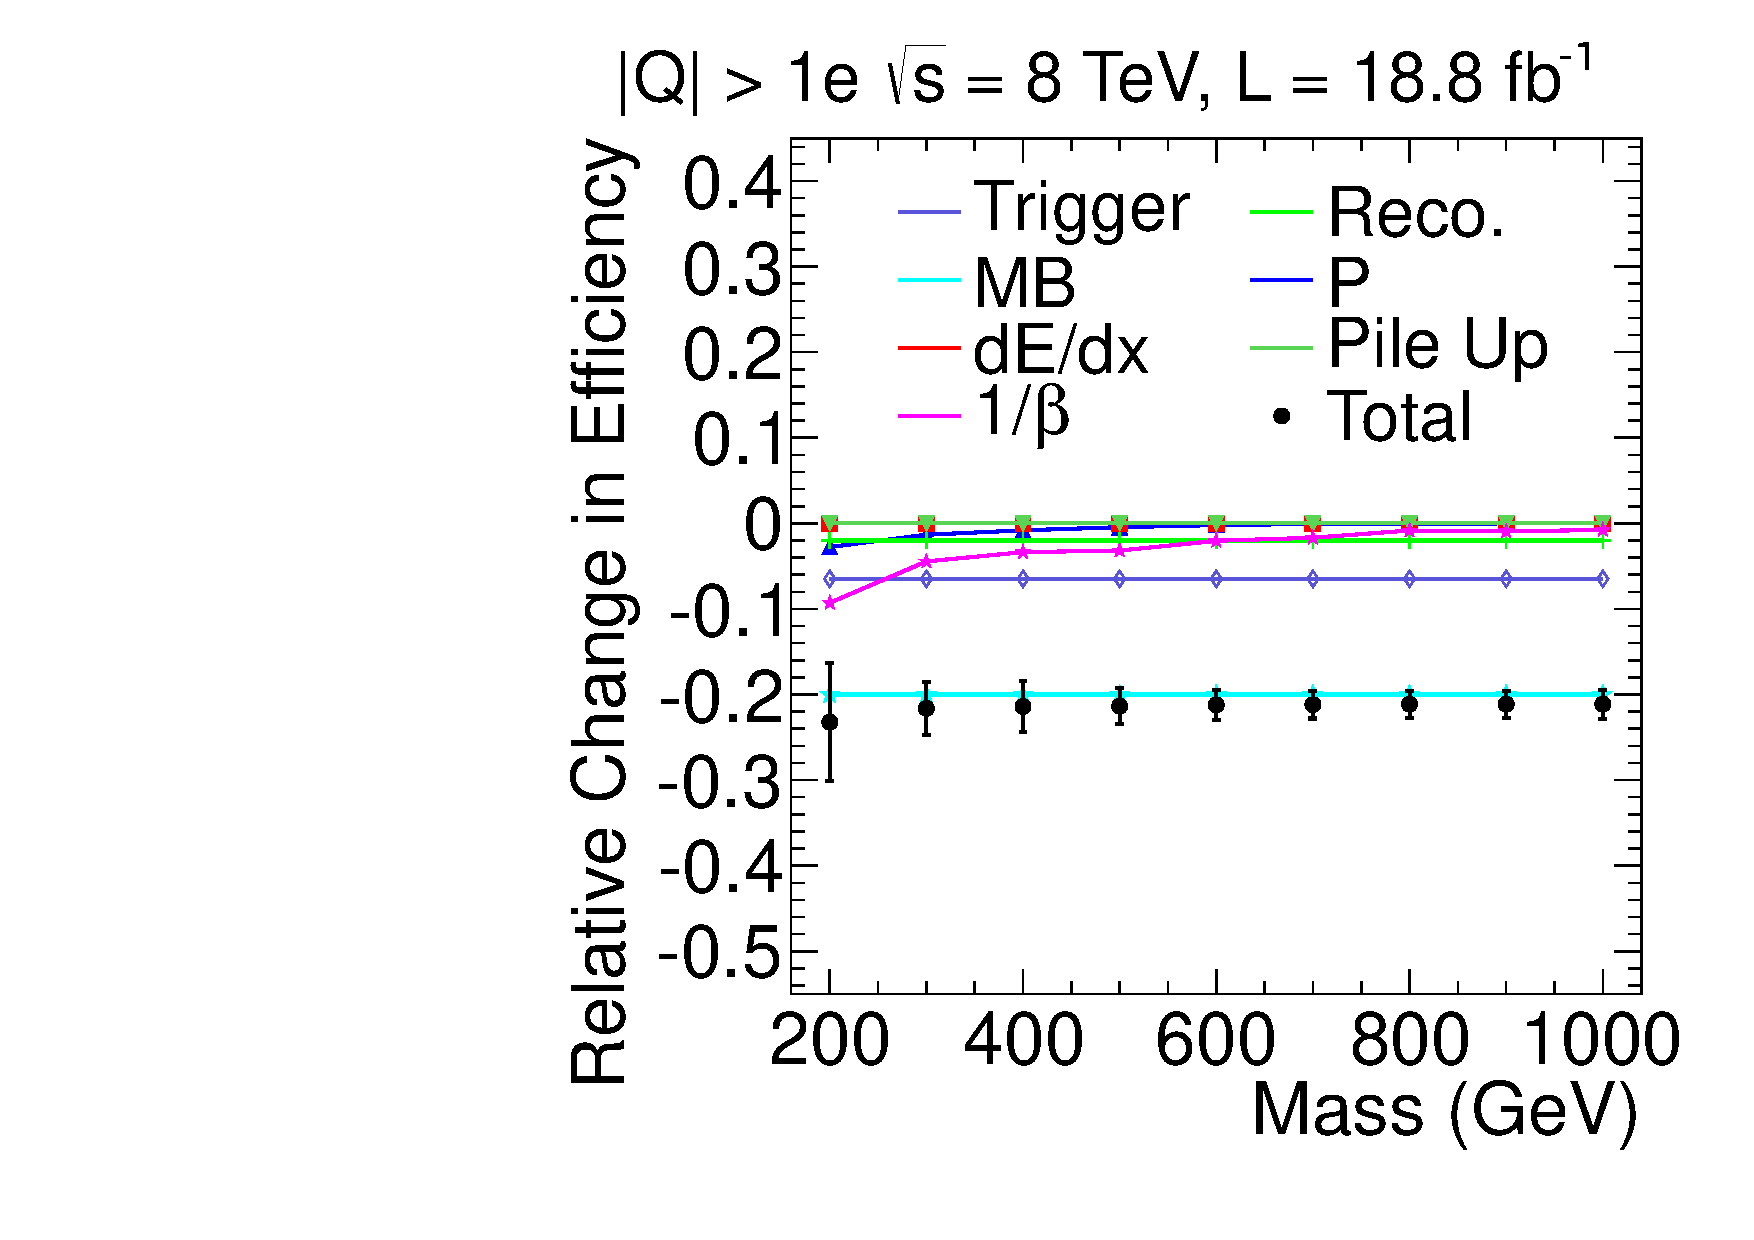
\includegraphics[clip=false, trim=0.0cm 0cm 0.0cm 0cm, width=0.48\textwidth]{figures/multi/HQDY_Q7Uncertainty}\\
\caption[Relative signal efficiency change seen for the various sources of uncertainty for some of the models considered in the \tkonly\ and \tktof\ analyses]
{Relative signal efficiency change seen for the various sources of uncertainty.
Error bars show only the statistical uncertainty.
Top row: Charge suppressed Gluino with $f=0.1$ (left) and charge suppressed stop (right) in the \tkonly\ analysis.
Bottom row: Q = 4e (left) and 7e (right) in the \multi\ analysis.}
    \label{fig:TkOnMCUncSource}
\end{figure}

The total signal efficiency uncertainty for all considered models is shown in
Figure~\ref{fig:TotalUnc} for the four analyses. The signal efficiency uncertainty used for each signal point is what is shown in this figure.
For all analyses except for the \multi\ analysis, the uncertainty is less than 15\% for all signal points and less than 10\% for a large majority of signal points.
For multiply charged samples, the uncertainty on the amount of detector material results in the total uncertainty to be between 20\% and 30\%.

\begin{figure}[ht]
\centering
  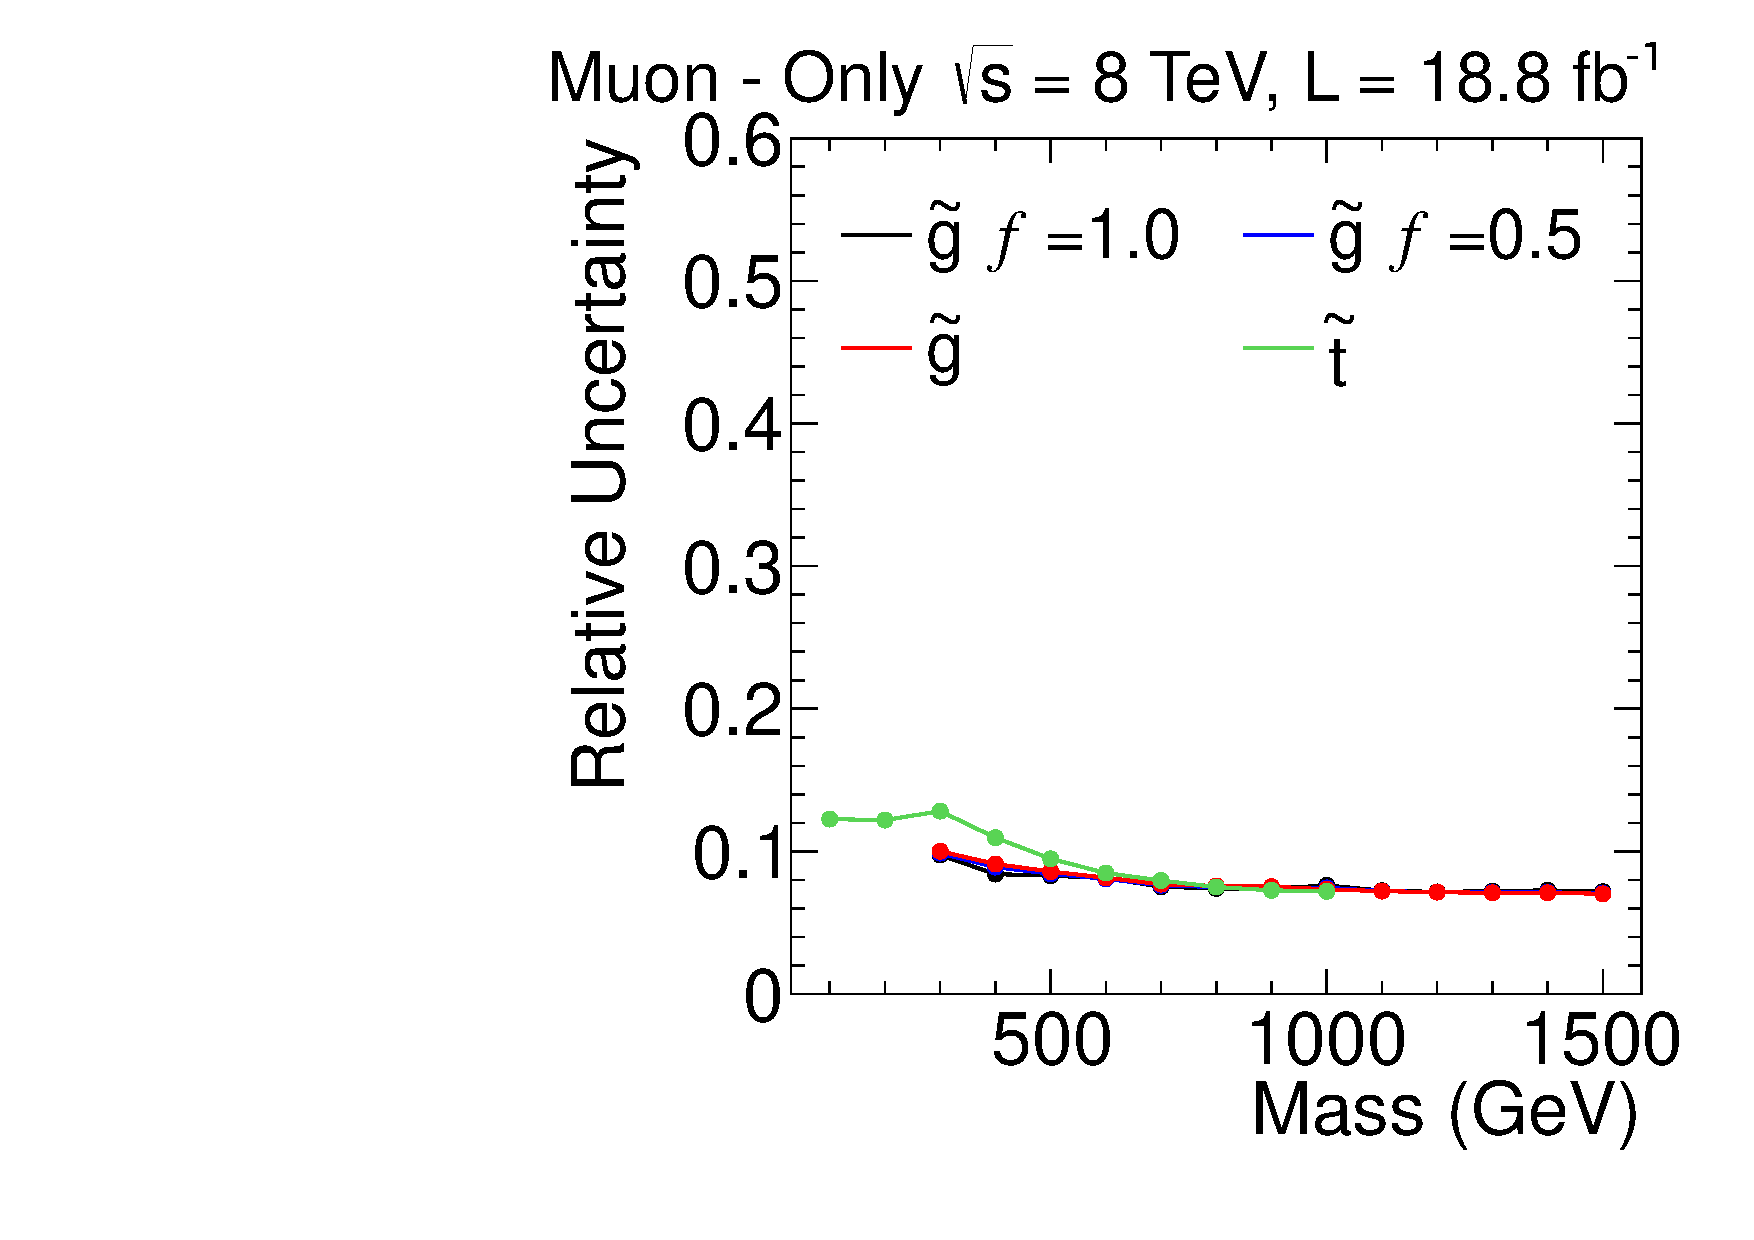
\includegraphics[clip=false, trim=0.0cm 0cm 0.0cm 0cm, width=0.48\textwidth]{figures/muonly/MOUncertainty}
  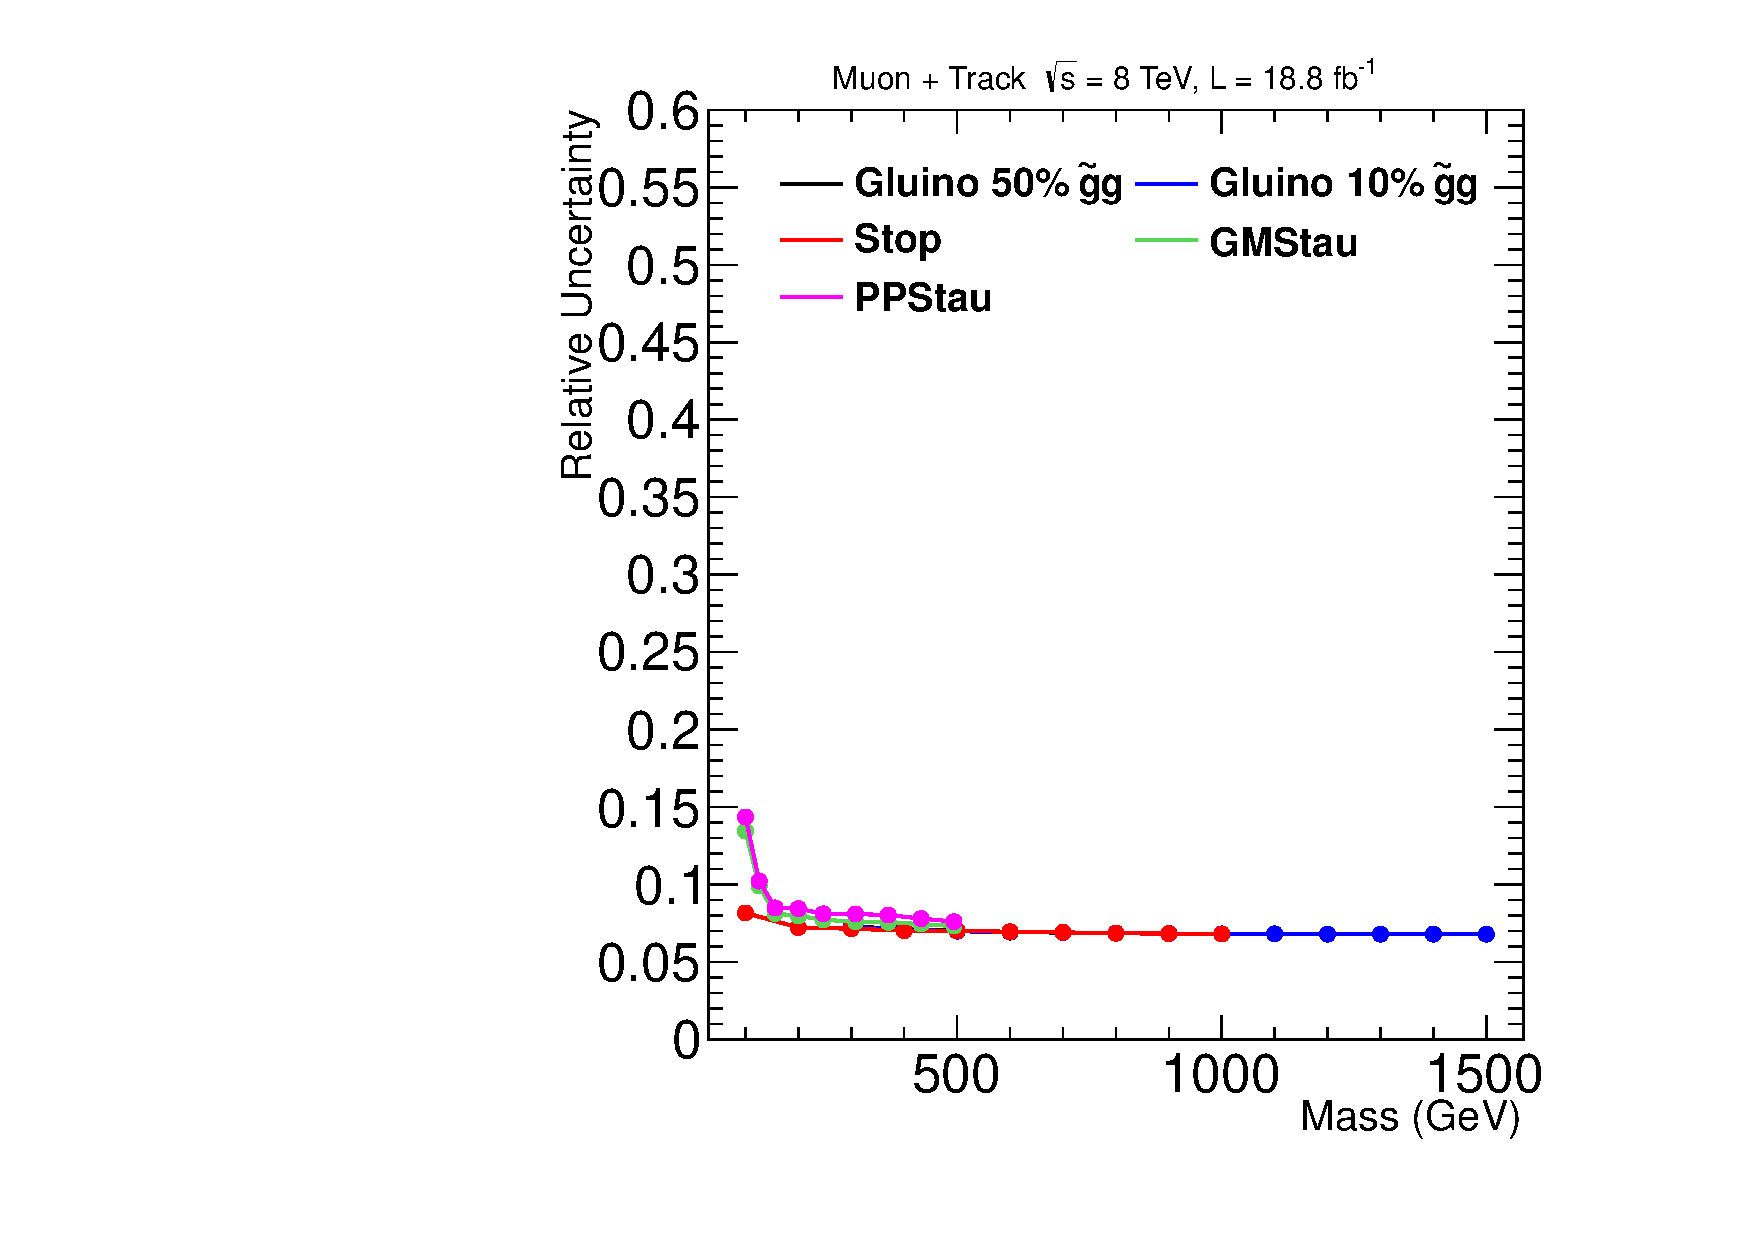
\includegraphics[clip=false, trim=0.0cm 0cm 0.0cm 0cm, width=0.48\textwidth]{figures/tkmu/MuUncertainty}
  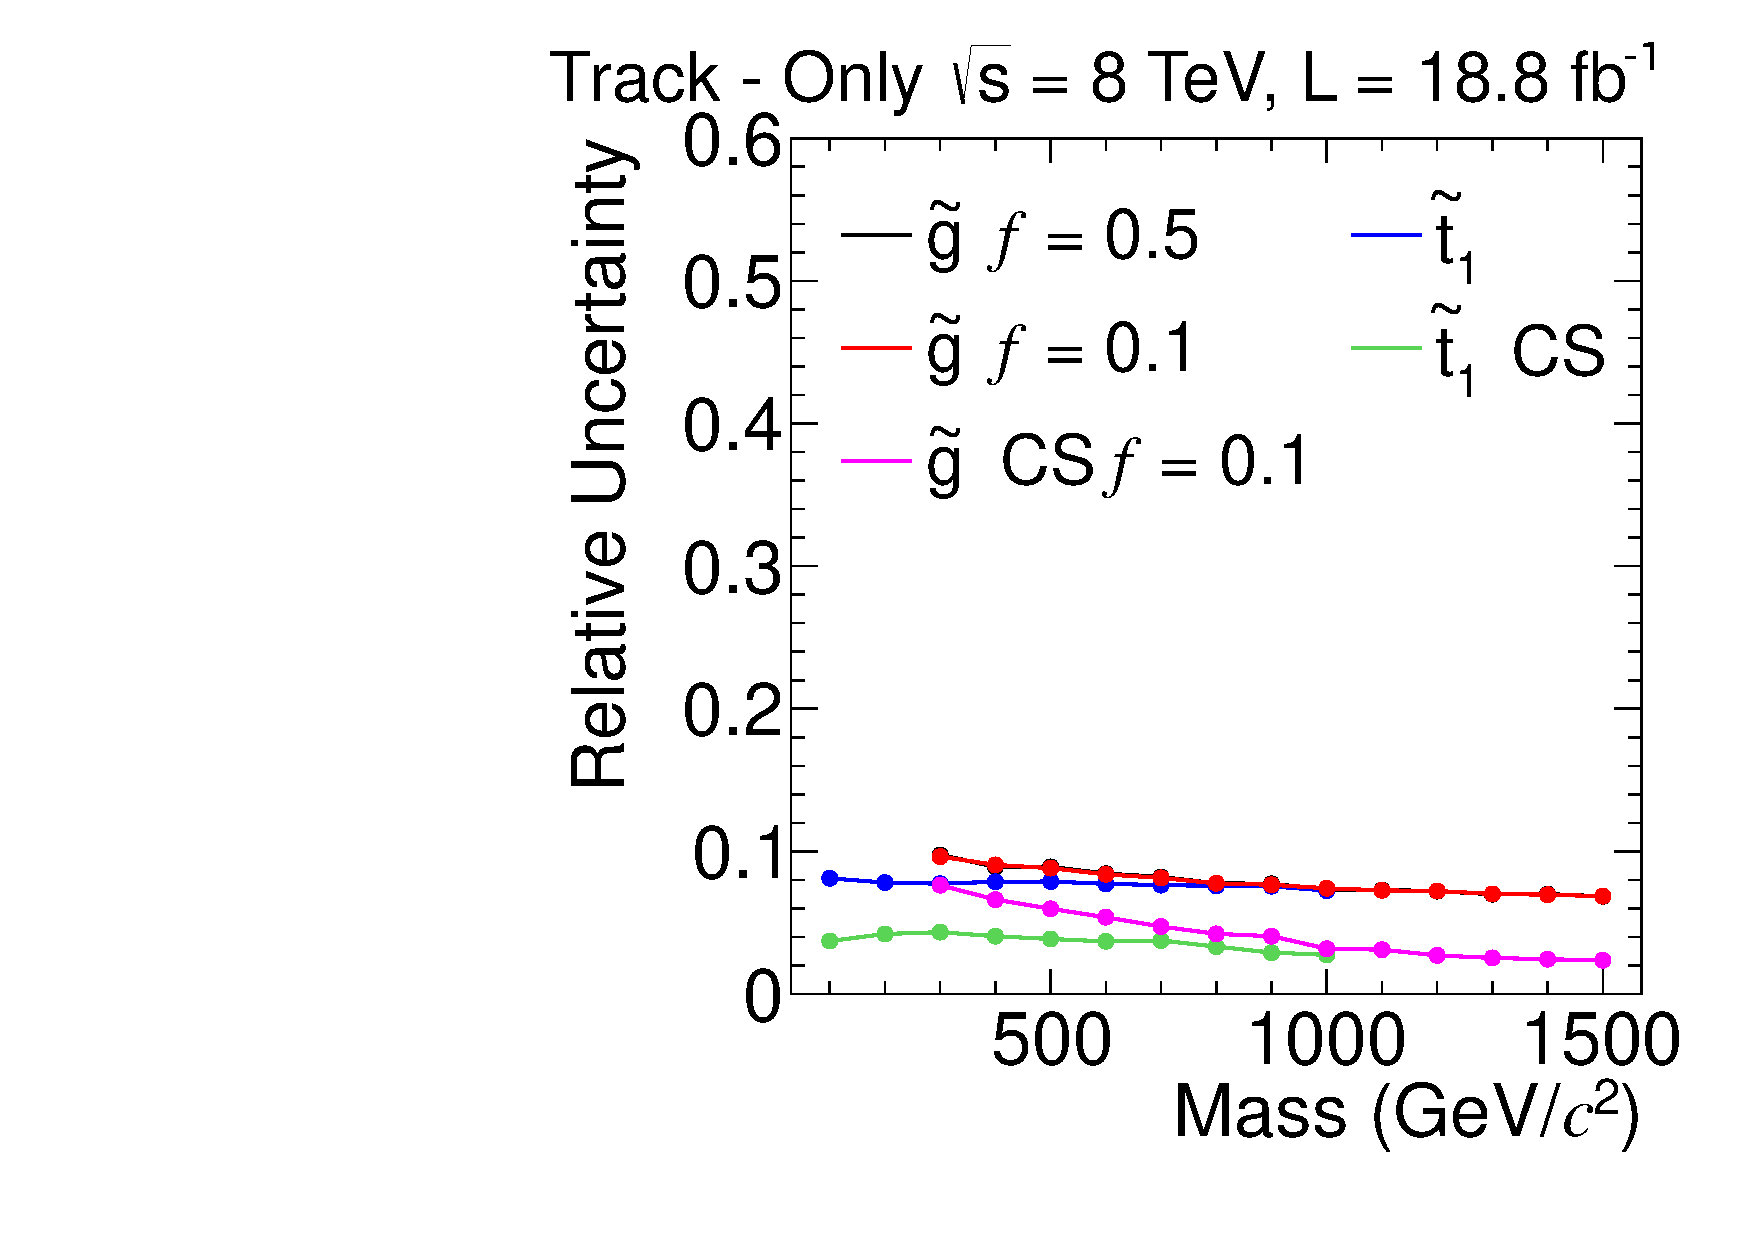
\includegraphics[clip=false, trim=0.0cm 0cm 0.0cm 0cm, width=0.48\textwidth]{figures/tkonly/TkUncertainty}
  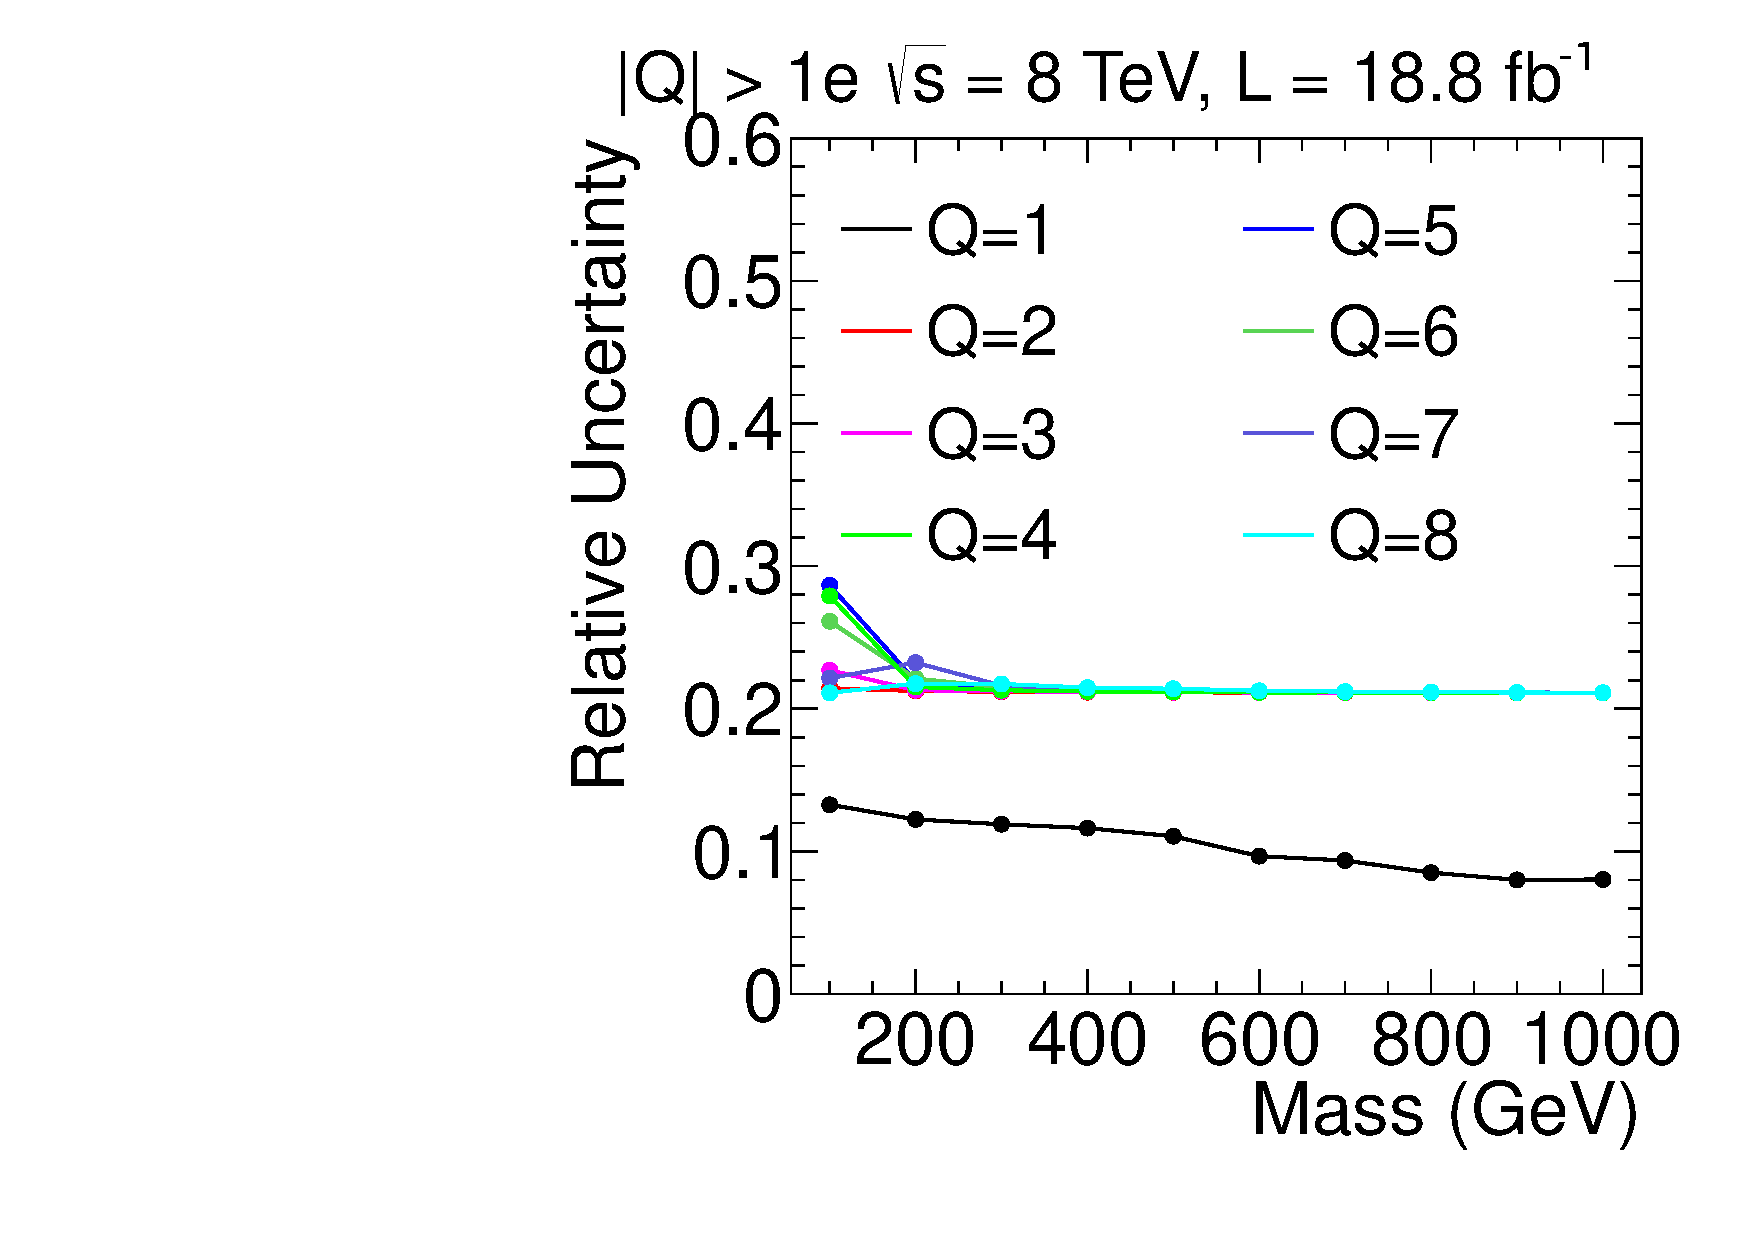
\includegraphics[clip=false, trim=0.0cm 0cm 0.0cm 0cm, width=0.48\textwidth]{figures/multi/HQUncertainty}
\caption[Total signal efficiency uncertainty for all considered models]
{Total signal efficiency uncertainty for all considered models.
Top:  For the \muononly\ (left) and \tktof\ (right) analyses.
Bottom:  For the \tkonly\ (left) and \multi\ (right) analyses.}
    \label{fig:TotalUnc}
\end{figure}

